\documentclass[10pt,letterpaper]{article}
\usepackage[top=0.85in,left=2.75in,footskip=0.75in]{geometry}

\usepackage{changepage}

\usepackage[utf8]{inputenc}

\usepackage{textcomp,marvosym}

\usepackage{fixltx2e}

\usepackage{amsmath,amssymb}

\usepackage{cite}

\usepackage{nameref,hyperref}

\usepackage[right]{lineno}

\usepackage{microtype}
\DisableLigatures[f]{encoding = *, family = * }

\usepackage{rotating}

\raggedright
\setlength{\parindent}{0.5cm}
\textwidth 5.25in 
\textheight 8.75in

\usepackage[aboveskip=1pt,labelfont=bf,labelsep=period,justification=raggedright,singlelinecheck=off]{caption}

% ==== begin added by me =====
\usepackage{svg}

\usepackage{float}

\usepackage[status=draft]{fixme}
\fxuselayouts{footnote,nomargin}

\usepackage{xstring}
\newcommand{\fillin}[1]{
    \IfEqCase{#1}{%
        {short}{\_}%
        {long}{\_\_\_\_\_}%
    }[\PackageError{fillin}{Undefined option to fillin: #1}{}]
}

\usepackage{nameref}

\graphicspath{{figures/}}
% ==== end added by me =====

\bibliographystyle{plos2015}

\makeatletter
\renewcommand{\@biblabel}[1]{\quad#1.}
\makeatother

\date{}

\usepackage{lastpage,fancyhdr,graphicx}
\usepackage{epstopdf}
\pagestyle{myheadings}
\pagestyle{fancy}
\fancyhf{}
\lhead{\includegraphics[width=2.0in]{PLOS-Submission.eps}}
\rfoot{\thepage/\pageref{LastPage}}
\renewcommand{\footrule}{\hrule height 2pt \vspace{2mm}}
\fancyheadoffset[L]{2.25in}
\fancyfootoffset[L]{2.25in}
\lfoot{\sf PLOS}

\newcommand{\lorem}{{\bf LOREM}}
\newcommand{\ipsum}{{\bf IPSUM}}

\begin{document}
\vspace*{0.35in}

% Title must be 250 characters or less.
% Please capitalize all terms in the title except conjunctions, prepositions, and articles.
\begin{flushleft}
{\Large
\textbf\newline{Applications of Machine Learning to Automated CFU Counting - Submission to PLOS Journals}
}
\newline
% Insert author names, affiliations and corresponding author email (do not include titles, positions, or degrees).
\\
Shea Conlon\textsuperscript{1} sheaconlon@berkeley.edu,
Will Ludington\textsuperscript{2} will.ludington@berkeley.edu
\\
\bigskip
\bf{1} Department of Computer Science, University of California at Berkeley, Berkeley, CA, USA
\\
\bf{2} Department of Molecular and Cell Biology, University of California at Berkeley, Berkeley, CA, USA
\\
\bigskip
\end{flushleft}
% Please keep the abstract below 300 words
\section*{Abstract}
    Counting colony-forming units (CFUs) on plates of growth medium is a necessary task in many microbiology experiments. Manual CFU counting has multiple drawbacks. First, its high cost in man-hours makes any experiment requiring large-volume CFU counting infeasible. Second, people may produce inconsistent counts, leading to poor data quality. This paper proposes automating CFU counting using machine learning approaches. Specifically, it demonstrates the use of deep convolutional neural networks to count via image segmentation and the use of support vector machines to count via image classification. It shows that these approaches improve the human cost and consistency of CFU counting and can generalize to different laboratory conditions.

\linenumbers

\section*{Introduction}
    Counting colony-forming units (CFUs) on plates of growth medium is a necessary task in many microbiology experiments, such as \fillin{long}. Manual CFU counting has the following drawbacks.

    \begin{enumerate}
        \item \textit{Lack of Scalability.}
            In our experience, it takes an average of $\fillin{short}$ minutes to manually count a single plate of $\fillin{short}$-$\fillin{short}$ CFUs. This high cost in man-hours makes large-volume CFU counting infeasible, restricting the types of experiments that can be performed. For example, without automating CFU counting, you could not count a large number of $96$-well plates (since each plate would require $96$ counts) and you could not produce fine-grain CFU growth curves (since each plate would require a count each hour).
        
        \item \textit{Lack of Consistency.}
            In our experience, CFU counts produced by different people differ significantly.\fxnote{Provide an image of a plate and two counts it was given?} This occurs because some plates are difficult and subjective to count; decisions must be made by the counter about which CFUs are small enough to ignore, which CFUs should be counted as two, which areas should be counted via density estimation instead of direct counting, etc. It is then desirable that for a given set of counts, either one person should do all of them (consistency via a "single source of truth") or two people should replicate all of them (consistency via replication and averaging). The first solution can cause a bottleneck in the experimental pipeline and contribute to the lack of scalability above. The second solution wastes time that could be spent doing better things. Automating the process imitates the first solution; a machine learning model can act as a "single source of truth" for counts. While the counts it produces will still be subjective, they will be self-consistent.
    \end{enumerate}
    
    \paragraph*{Related Work.}
        Related work in this area has focused on the segmentation of organs in biomedical images \cite{Novikov, Ronneberger} and cells in microscope images \cite{Valen}. Some has addressed CFU counting, but in the clinical laboratory setting, where conditions are tightly controlled and there are large volumes of data available \cite{Ferrari}. This paper applies the core model\fxnote{Tune Valen et al.'s architecture specifically for this use case.} of \cite{Valen} to CFU counting in the scientific laboratory, where conditions vary widely and data is not readily available. It then analyzes the model's ability to generalize to new conditions and adds measures to make the model reusable by other labs with minimal tuning. Finally, it presents an alternative model for CFU counting that is faster to train and use, along with measures for handling its decreased accuracy.

\section*{Materials and Methods}
    Subsection \textit{Datasets} describes the datasets used in our experiments. Subsection \textit{DCNN} describes the methodology behind the deep convolutional neural network used for counting CFUs via image segmentation. Subsection \textit{SVM} describes the methodology behind the support vector machine used for counting CFUs via image classification.
    
    \subsection*{Datasets} \label{ssec:datasets}
        \paragraph*{Image Masks.}
            Going forward, we will refer to "masks" of images. A mask $M$ for condition $c$ of an image $I$ is itself an image of the same dimensions as $I$. $M$'s pixel at $(x, y)$ is black if $c$ is true of $I$'s pixel at $(x, y)$ and white otherwise. For example, in the inside-a-CFU mask for a plate image, the mask's pixel at $(x, y)$ is black if the plate's pixel at $(x, y)$ is inside a CFU and white if it is outside all CFUs.

        \paragraph*{\texttt{easy\_masked} Dataset}
            This dataset consists of $2$ plate images, their masks, and their counts. The masks mark the pixels that are inside a CFU, on the edge of some CFU(s), and outside all CFUs. The plate images were captured with a typical smartphone ($2448px \times 3264px$, RGB) and no special setup. The masks were drawn by hand using Adobe Photoshop and a graphics tablet. The counts were collected according to the usual practices of the group. One example can be seen in Fig.~\ref{easy-masked}. This dataset is used for training the DCNN.

            \begin{figure}[h]
                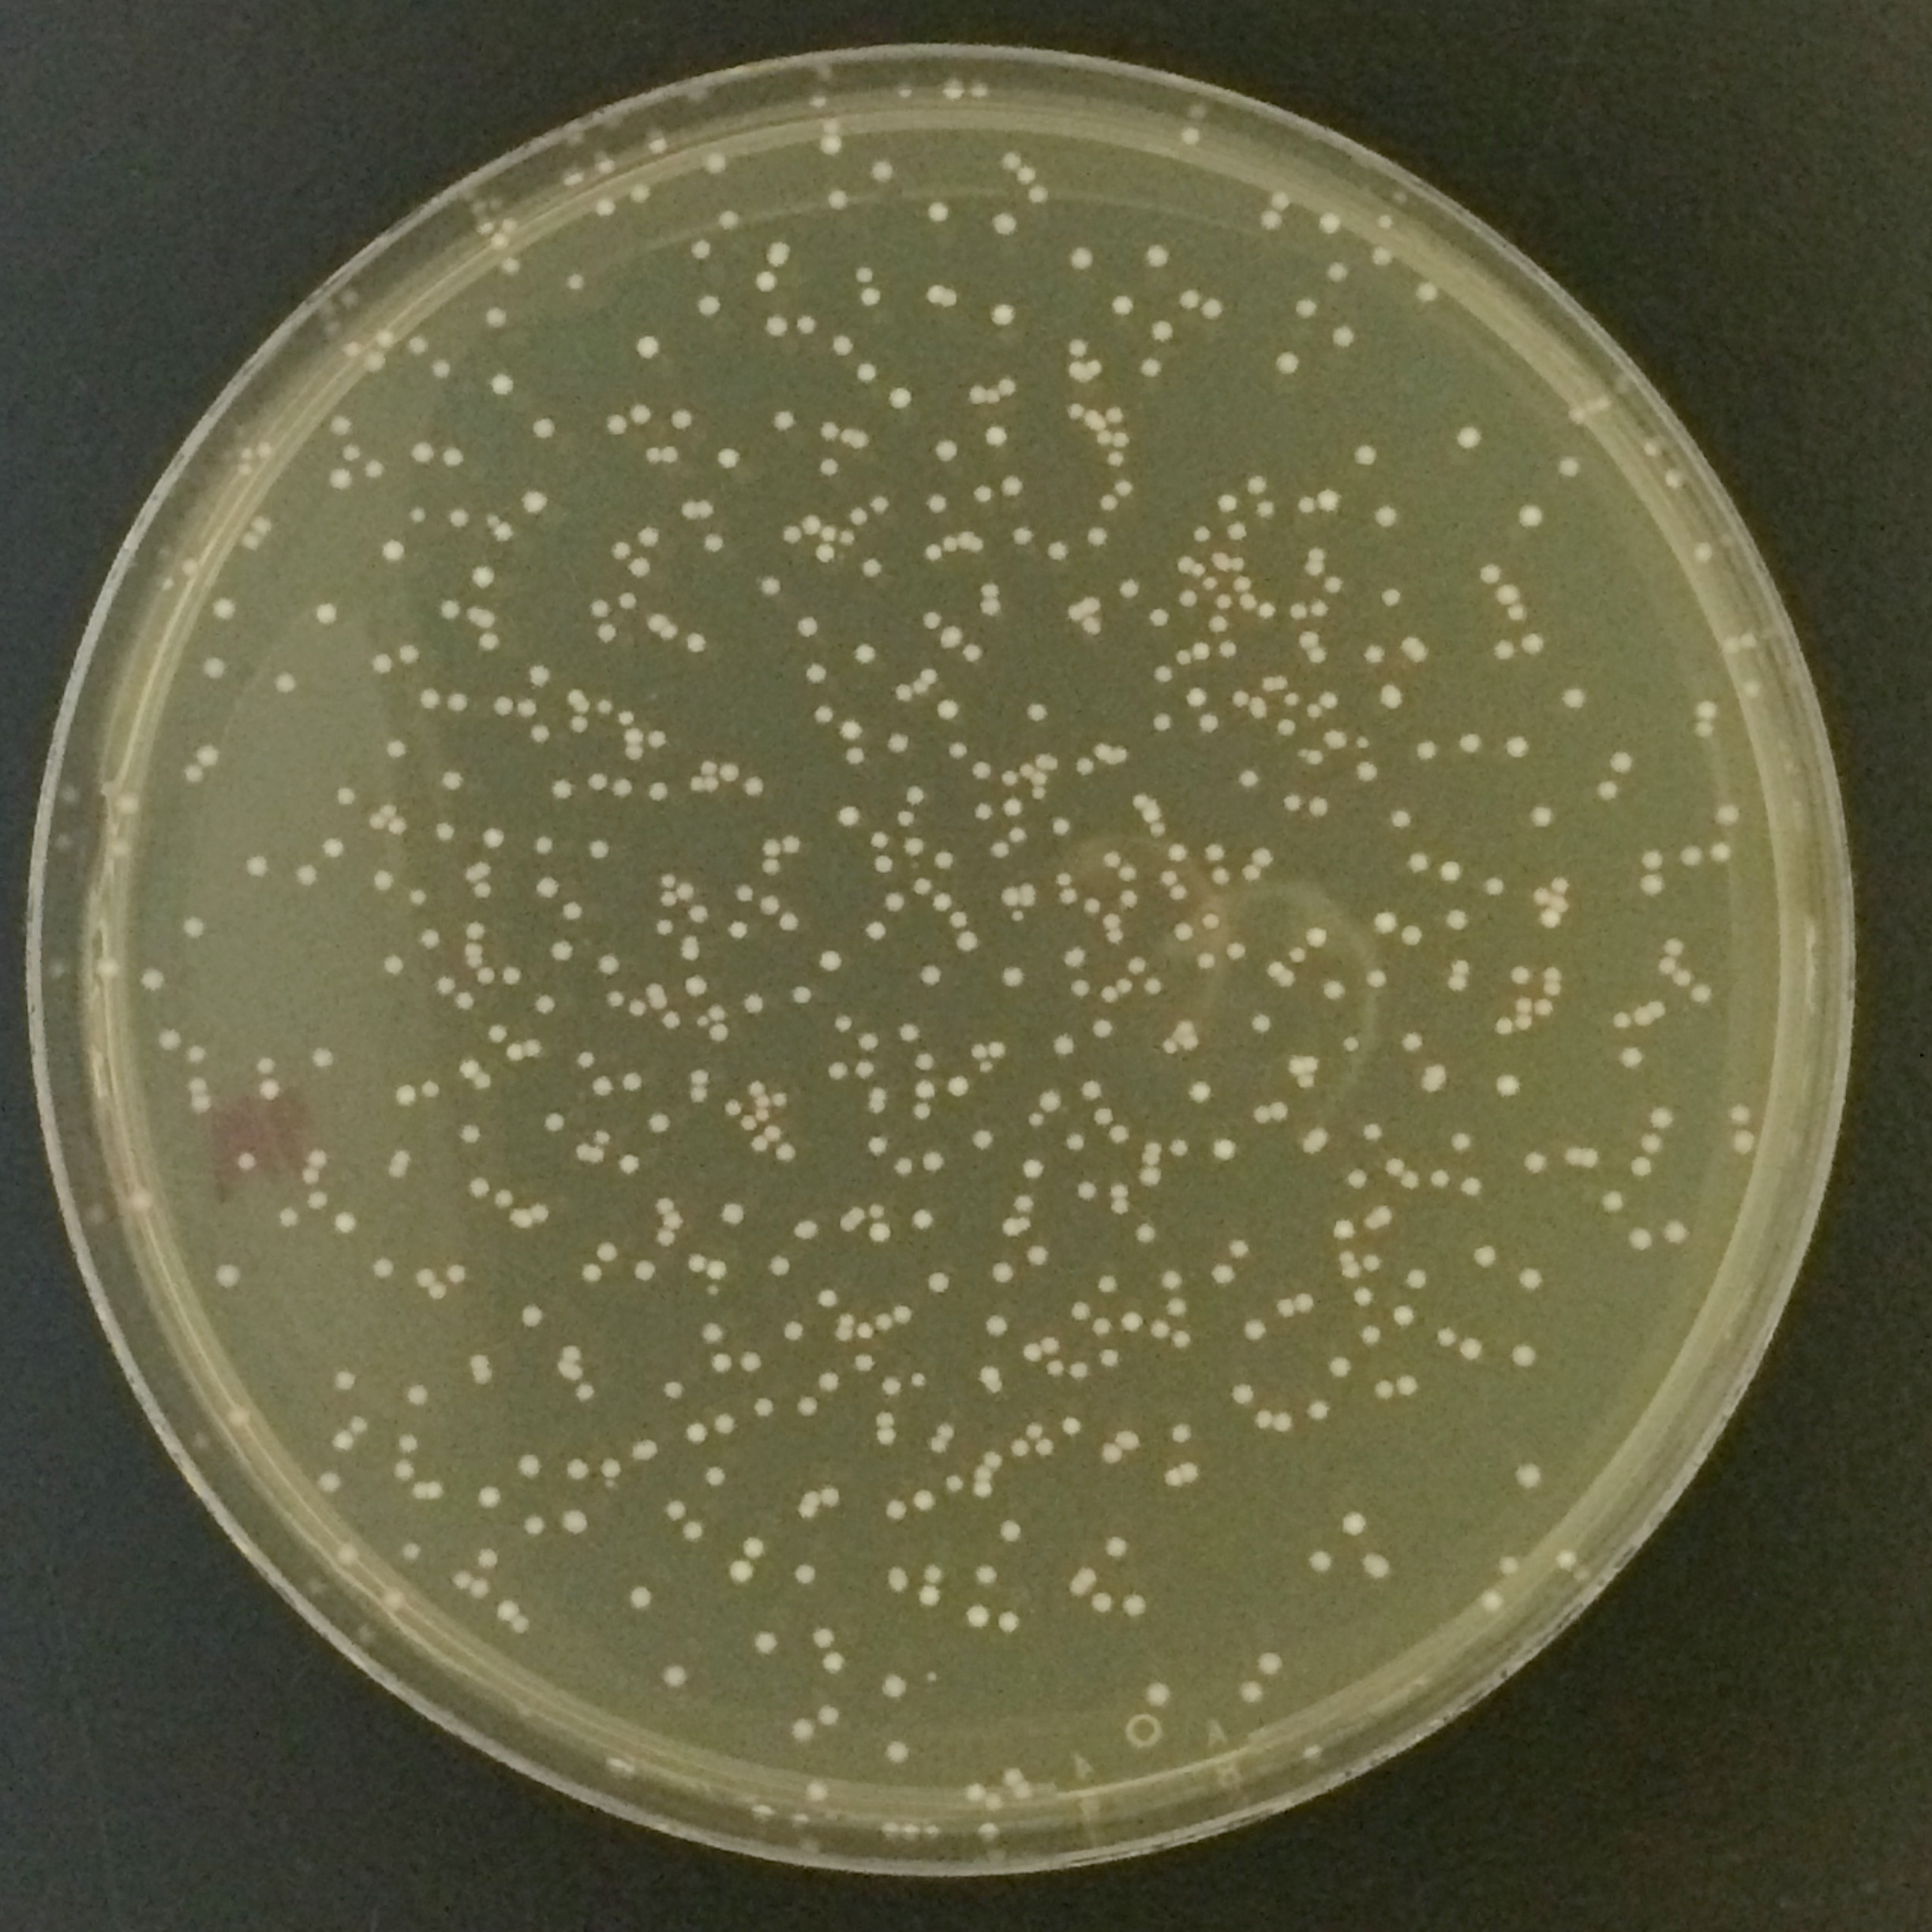
\includegraphics[width=0.2\textwidth]{easy_0_image}
                \includegraphics[width=0.2\textwidth]{easy_0_inside}
                \includegraphics[width=0.2\textwidth]{easy_0_edge}
                \includegraphics[width=0.2\textwidth]{easy_0_outside}
                \caption{{\bf Example of \texttt{easy\_masked} Dataset.} From left to right is the plate image, its \texttt{inside}-CFU mask, its \texttt{edge}-of-CFU mask, and its \texttt{outside}-all-CFUs mask.}
                \label{easy-masked}
            \end{figure}

        \paragraph*{\texttt{more\_masked} Dataset}
            This dataset contains the same components as $\texttt{easy\_masked}$. It has only $1$ plate, of a different bacterial strain, whose colonies have different size and morphology. It can be seen in Fig.~\ref{more-masked}. This dataset is used for training the DCNN.
        
            \begin{figure}[h]
                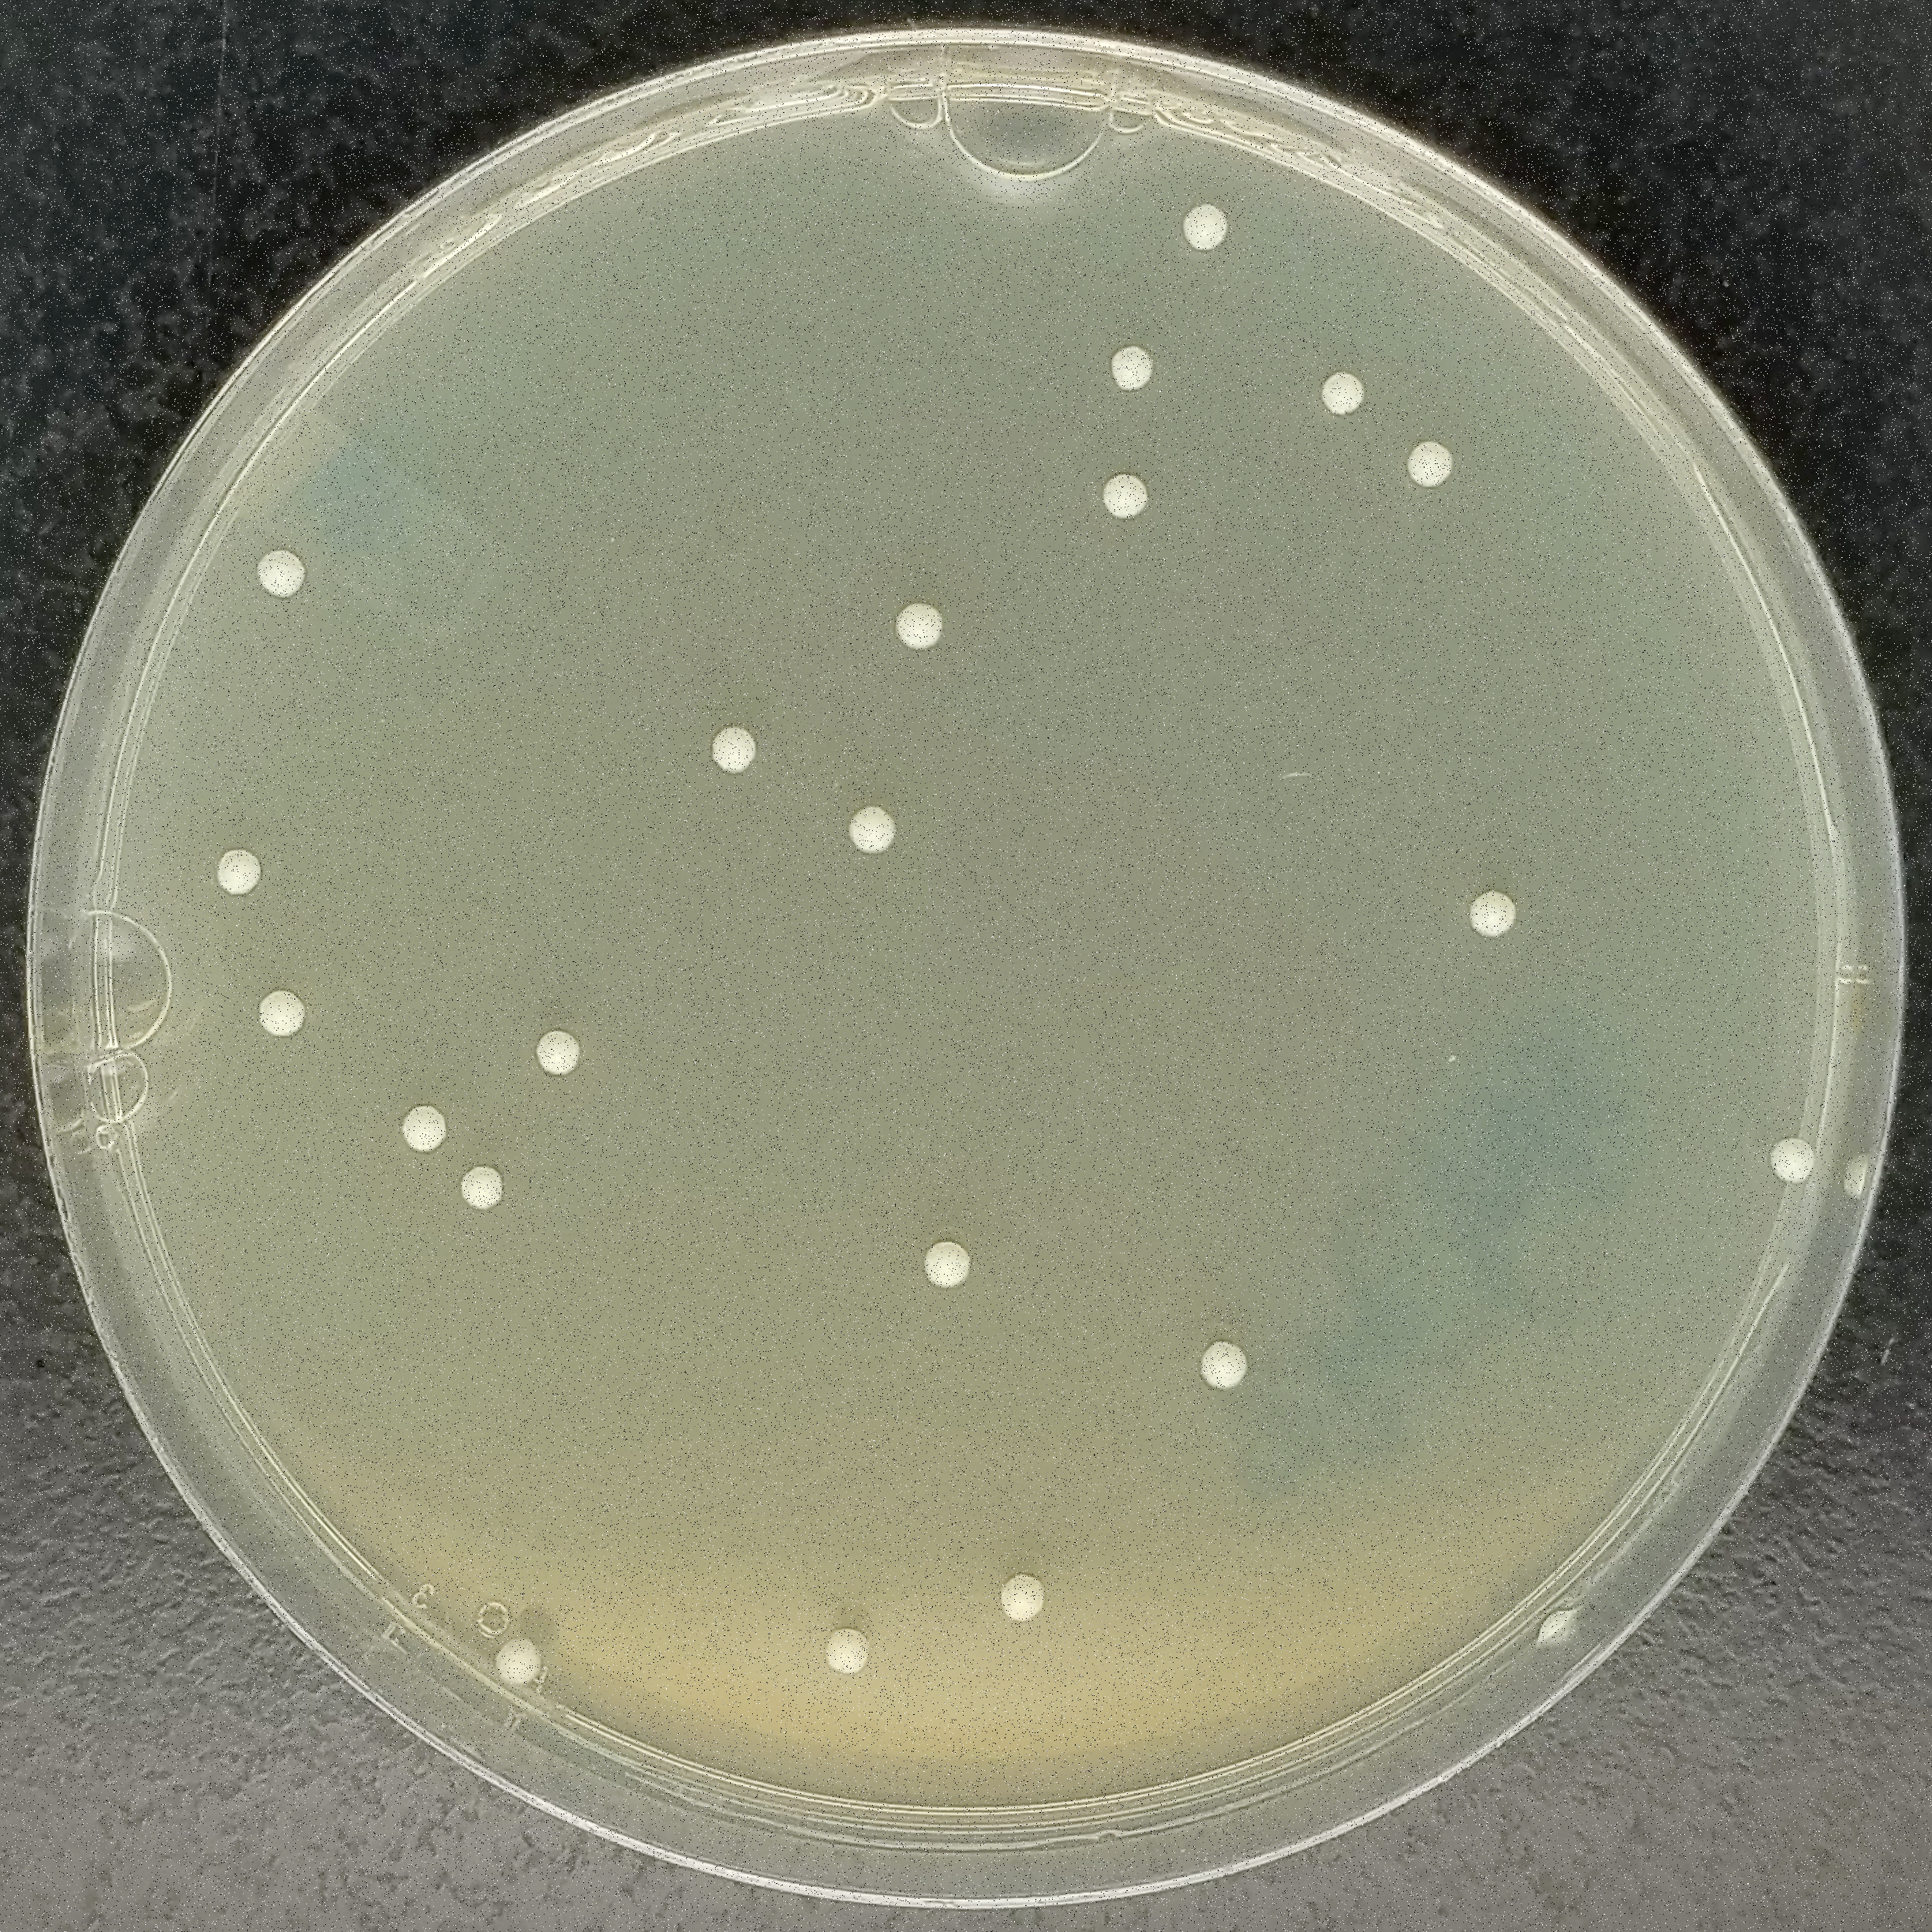
\includegraphics[width=0.2\textwidth]{more_0_image}
                \includegraphics[width=0.2\textwidth]{more_0_inside}
                \includegraphics[width=0.2\textwidth]{more_0_edge}
                \includegraphics[width=0.2\textwidth]{more_0_outside}
                \caption{{\bf Example of \texttt{more\_masked} Dataset.}}
                \label{more-masked}
            \end{figure}

        \paragraph*{\texttt{easy} Dataset}
            This dataset consists of $26$ plate images and their counts. It comes from the same batch of plates (with the same bacterial strain) as $\texttt{easy\_masked}$. The only difference is no masks have been made for these. This dataset is used for testing the DCNN.
            
        \paragraph*{\texttt{more} Dataset}
            This dataset consists of $2$ plate images and their counts. It comes from the same batch of plates (with the same bacterial strain) as $\texttt{more}$. The only difference is no masks have been made for these. This dataset is used for testing the DCNN.

        \paragraph*{\texttt{multi} Dataset}
            This dataset consists of $3$ plates images, each photographed under $3$ conditions, as well as the plates' counts. The conditions are listed below. It can be seen in Fig.~\ref{multi}. This dataset is used for testing the DCNN.

            \begin{enumerate}
                \item $\texttt{light\_uncovered\_far\_noperspective}$: Photographed with extra lighting, with the plate's cover removed, from about $1ft$ away, with no perspective
                \item $\texttt{nolight\_uncovered\_close\_minorperspective}$: Photographed without extra lighting, with the plate's cover removed, from about $3in$ away, with minor perspective
                \item $\texttt{light\_covered\_close\_severeperspective}$: Photographed with extra lighting, with the plate's cover on, from about $3in$ away, with severe perspective.
            \end{enumerate}
            
            \begin{figure}[h]
                \includesvg[svgpath=figures/, width=0.7\textwidth]{plate_0}
                \caption{{\bf Example of \texttt{multi} Dataset.}}
                \label{multi}
            \end{figure}

        \paragraph*{\texttt{pinned} Dataset}    
            This dataset consists of $417$ well images and their counts. The well images are extracted from a set of $32$ images of 96-well plates. It can be seen in Fig.~\ref{pinned}. This dataset is used for testing the DCNN, as well as training, validating, and testing the SVM.
            
            \begin{figure}[h]
                \includesvg[svgpath=figures/, width=0.7\textwidth]{plates_resized}
                \caption{{\bf Sample of \texttt{pinned} Dataset.}}
                \label{pinned}
            \end{figure}

    \subsection*{DCNN} \label{ssec:dcnn}
        \paragraph*{Summary}
            Our first model is a deep convolutional neural network (DCNN) that copies the architecture of \cite{Valen}. In brief, the model takes as input a $61px \times 61px$ image. It outputs a "class", one of \texttt{inside}, \texttt{edge}, or \texttt{outside}. Our goal is to be able to input a $61px \times 61px$ patch of a plate image and have the DCNN output whether the center pixel of the patch is \texttt{inside} a CFU, on the \texttt{edge} of some CFU(s), or \texttt{outside} all CFUs. We will then collect the \texttt{inside} classifications into an \texttt{inside}-a-CFU mask of the image, which constitutes a segmentation of the image. Then, we will use standard algorithms to clean up noise and count the number of segments present. This pipeline is depicted in Fig.~\cite{dcnn_pipeline}.
            
            \begin{figure}[h]
                \includegraphics[width=0.7\textwidth]{dcnn_pipeline2}
                \fxnote{Clean this up.}
                \caption{{\bf DCNN Pipeline.} Each pixel of a plate image is classified as either \texttt{inside}, \texttt{edge}, or \texttt{outside} by the DCNN in order to produce a segmentation mask.}
                \label{dcnn_pipeline}
            \end{figure}
        
    
        \paragraph*{Model Overview}
            We present an overview of some key concepts relating to DCNNs below. Specific details on its architecture can be found in \nameref{S1_Text}.
        
            \begin{itemize}
                \item
                    \textit{Neural network.} A neural network is a mathematical object that accepts some inputs and returns some outputs. Neurons in a neural network loosely model biological neurons; they sum up the signals that come in through their input connections, apply a function to the sum, and output the result along their output connections. Connections have strengths which we call weights. Suppose we arranged multiple of these neurons side-by-side in a layer. Mathematically, if the inputs to the network were contained in the vector $x$, the weights of the connections from each input to each neuron were contained in the matrix $W$, and the function the neurons apply were $f$, then the outputs of the neurons would be $f(W \cdot x)$. This situation is depicted in Fig.~\ref{dcnn_neural_network}. Intuitively, by setting up neural networks in this relatively unstructured manner, we give them considerable flexibility to represent a wide class of relationships between their inputs and outputs, depending on the tuning of their weights.
            
                    \begin{figure}[h]
                        \includegraphics[width=0.7\textwidth]{dcnn_neural_net}
                        \caption{{\bf Neural Network.} Only the connection between input $6$ and neuron $2$ (with weight $w_{2, 6}$) is visualized, but in reality there is a connection between each input and each neuron (each with its own weight $w_{i, j}$).}
                        \label{dcnn_neural_network}
                    \end{figure}
            
                \item
                    \textit{Deep.}
                        A deep neural network is a neural network with multiple layers of neurons. In a deep neural network, the inputs of layer $i$ are the outputs of layer $i - 1$. Denoting the matrix of weights coming into layer $i$ as $W_i$, the output of the entire network is the output of the last layer, which is $f(f(\ldots f(x \cdot W_1) \ldots \cdot W_{n-1}) \cdot W_n)$. Intuitively, by stacking these layers, we give the network the power to represent more complex relationships between its inputs and outputs using hierarchical representation.
            
                \item
                    \textit{Convolutional.}
                        A convolutional neural network converts the first few layers of the network into convolutional layers which use a different interconnection structure. Instead of connecting each input $i$ to each neuron $j$ using an independent weight $w_{i,j}$, a convolutional layer uses a much smaller number of weights and reuses those same weights on each spatial patch of the input. It is most commonly used when the input is an image. Intuitively, when the input is an image, sharing the same weights across each patch of the image enforces the extraction of the same location-invariant information from each patch of the image, at least in the first few layers of the network.
                
                \item
                    \textit{Training.}
                        When a neural network is trained, it is made to produce outputs that, approximately, have some desired relationship with the network's inputs. Training requires a training dataset of both inputs $\{x_1, \ldots, x_n\}$ and their correct outputs $\{y_1, \ldots, y_n\}$, typically containing on the order of at least $100,000$ examples. You feed the network the inputs $x_i$, obtain using the weights $W$ some outputs $\hat{y_i}$ which are interpreted as predicting the correct outputs, and calculate the sum of errors of the predictions, something like $\sum_{i = 1}^n (\hat{y_i} - y_i)^2$. You take the derivative of the error with respect to the weights $\Delta_W (y_i - \hat{y_i})$ and adjust the weights slightly in the direction that reduces this error $W \gets W - 0.01\Delta_W (y_i - \hat{y_i})$. Then you repeat. Over time, the prediction error produced by the weights decreases and the network's outputs become better and better approximations for the correct outputs.
                \item
                    \textit{Avoiding Overfitting.}
                        In order to avoid overfitting, a term proportional to the square of the sizes of the weights is added to the loss. This encourages the use of small weights, which are less likely to memorize data and more likely to learn relationships. We additionally use batch normalization, a technique which normalizes each batch of data as it passes through the layers of the network and also helps to avoid overfitting \cite{Ioffe}.
            \end{itemize}

        \paragraph*{Preprocessing}
            The DCNN is trained and validated using a dataset that combines $\texttt{easy\_masked}$ and $\texttt{more\_masked}$. Preprocessing involves a number of steps, notably image normalization as in \cite{Valen} and data augmentation. Image normalization and data augmentation help to ensure the model learns the underlying structure of the problem instead of relying on the brightness or color of the center pixel, since that may vary between experiments, be affected by photographic conditions, or be misleading due to noise.
    
            \begin{enumerate}
                \item
                    We augment the dataset by duplicating each image $10$ times, then randomly modifying the resulting images. With $25\%$ probability, a given image is flipped horizontally, flipped vertically, or perspective distorted. With $5\%$ probability, a given image gets a random value added to it, gets blurred a random amount, gets random Gaussian noise added to it, gets black and white pixels substituted into it, gets contrast normalized by a random amount, or gets desaturated by a random amount. With $2\%$ probability, a given image gets inverted, gets its hue and saturation changed by a random amount, or gets sharpened by a random amount. An example can be seen in Fig.~\ref{dcnn_augmentation_mutation}.
        
                \begin{figure}[h]
                    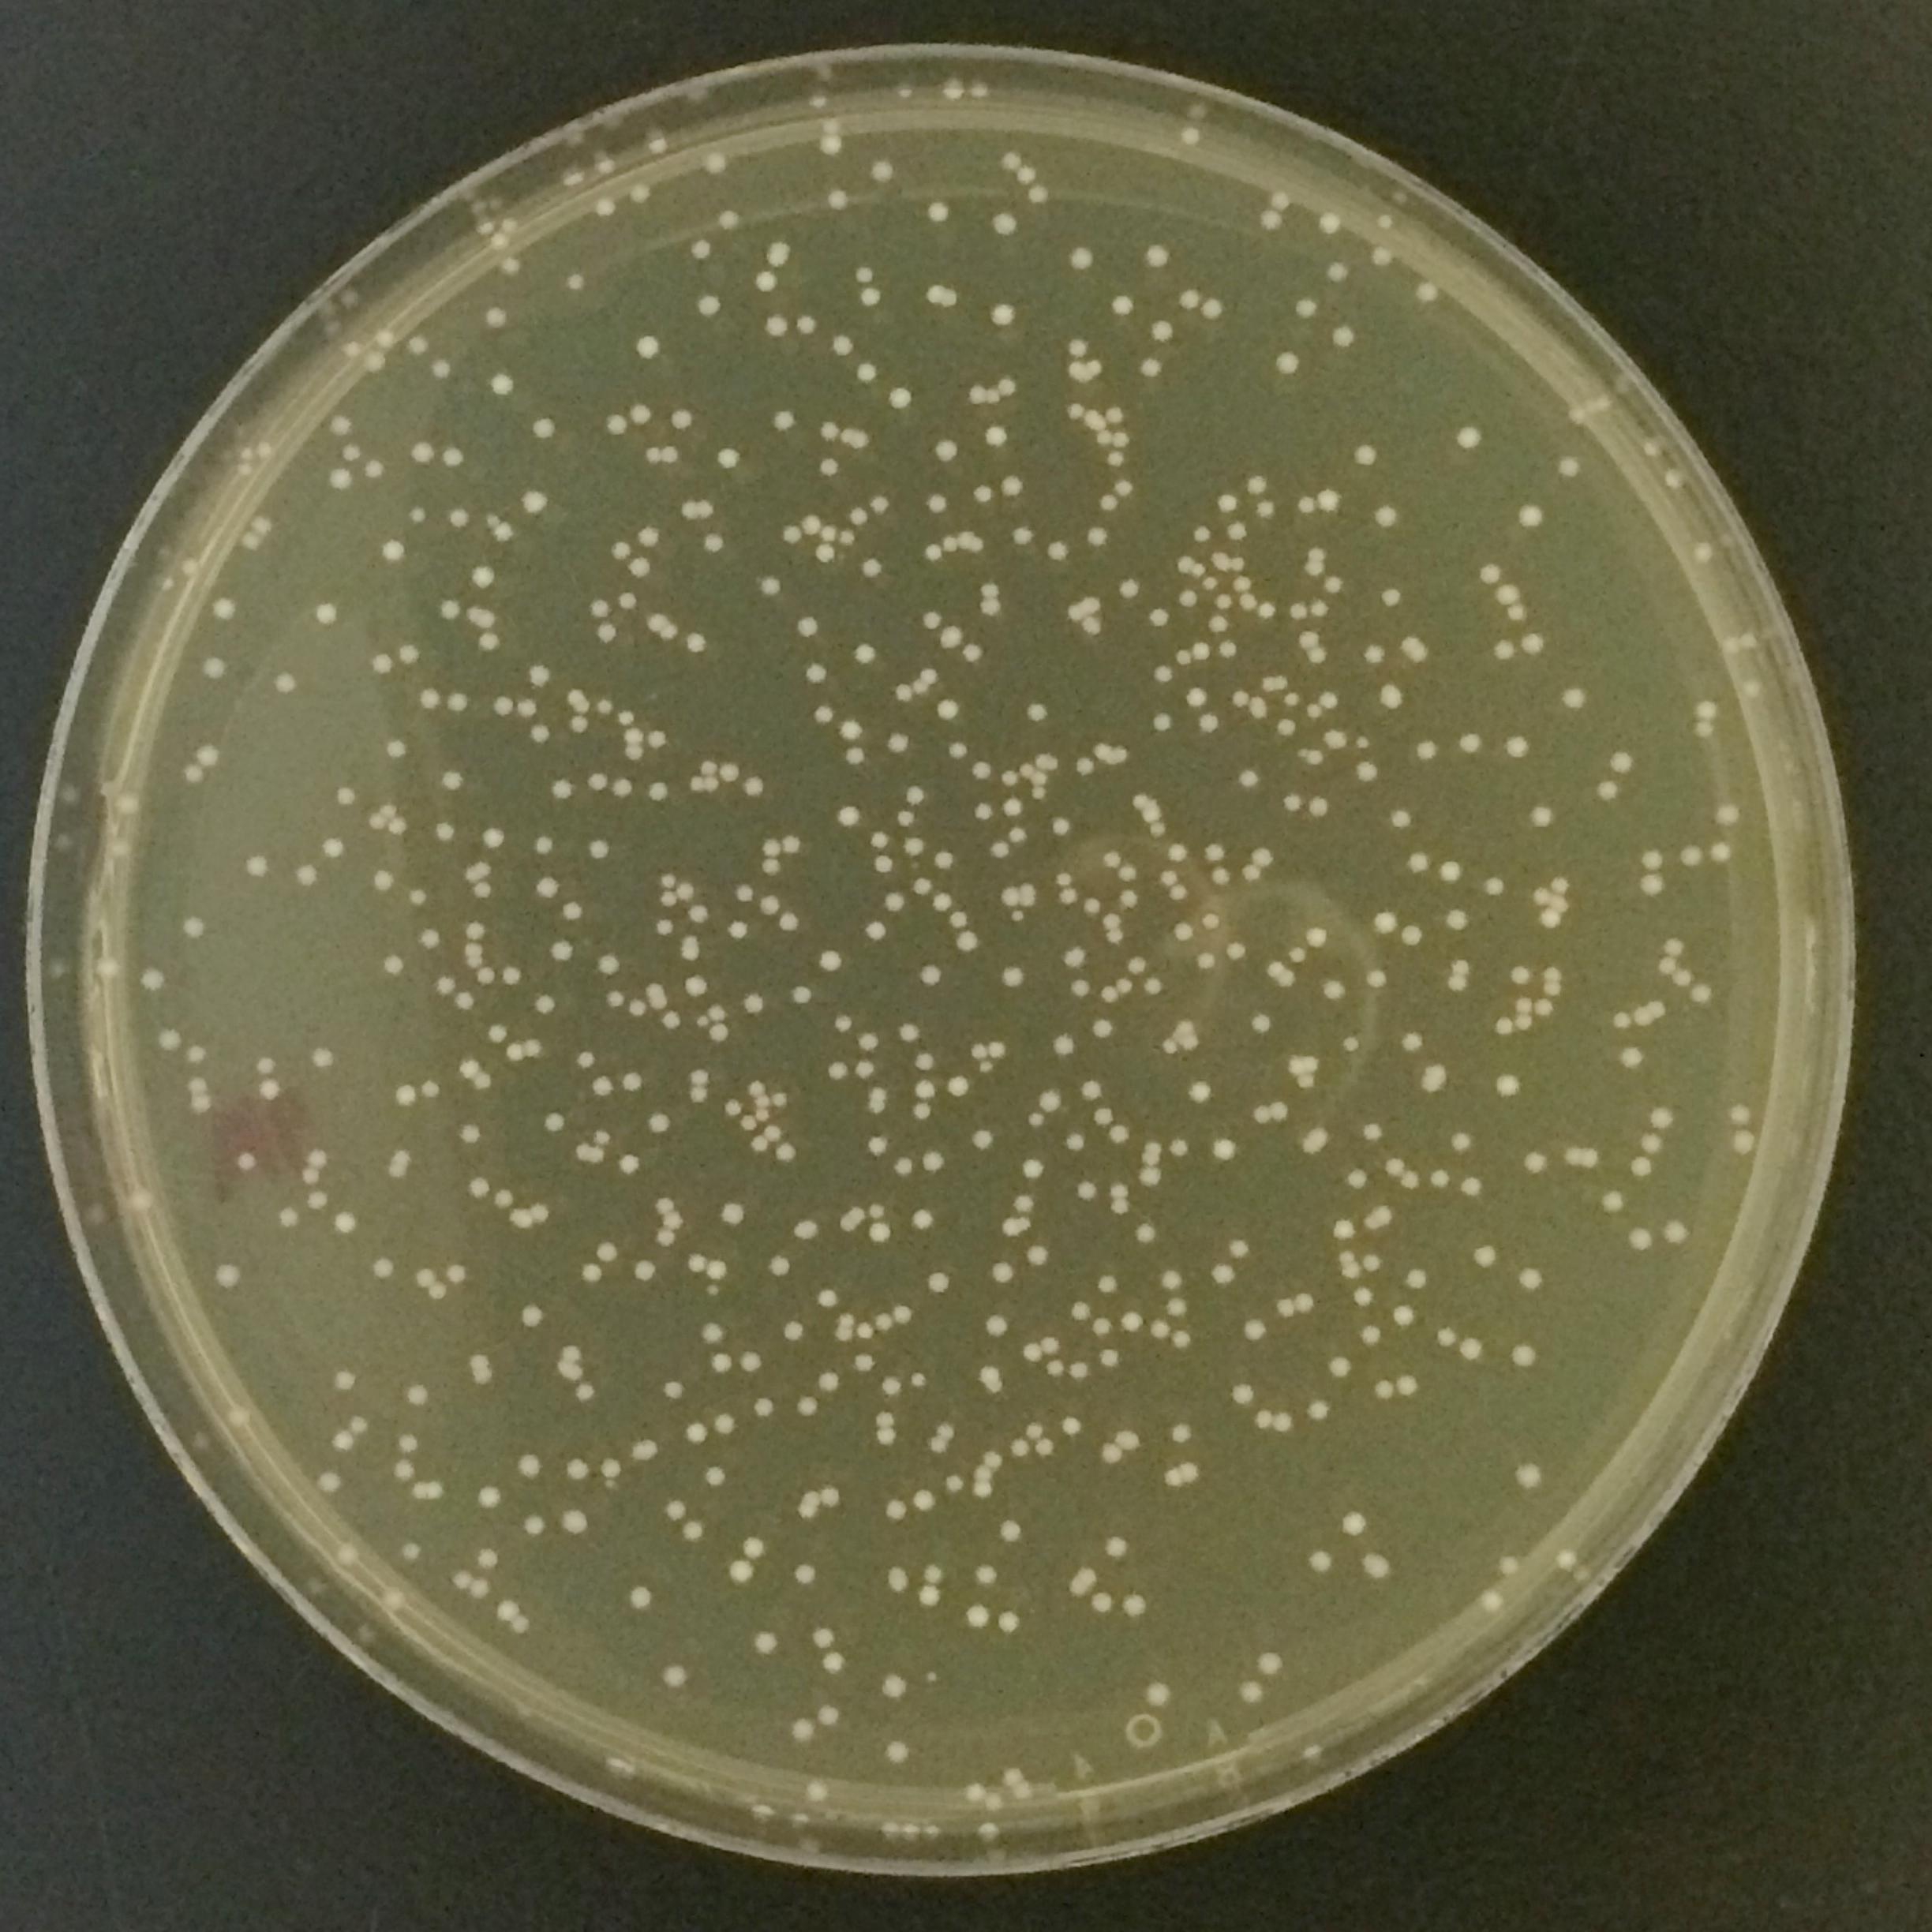
\includegraphics[width=0.25\textwidth,resolution=300]{original_easy_0_image}
                    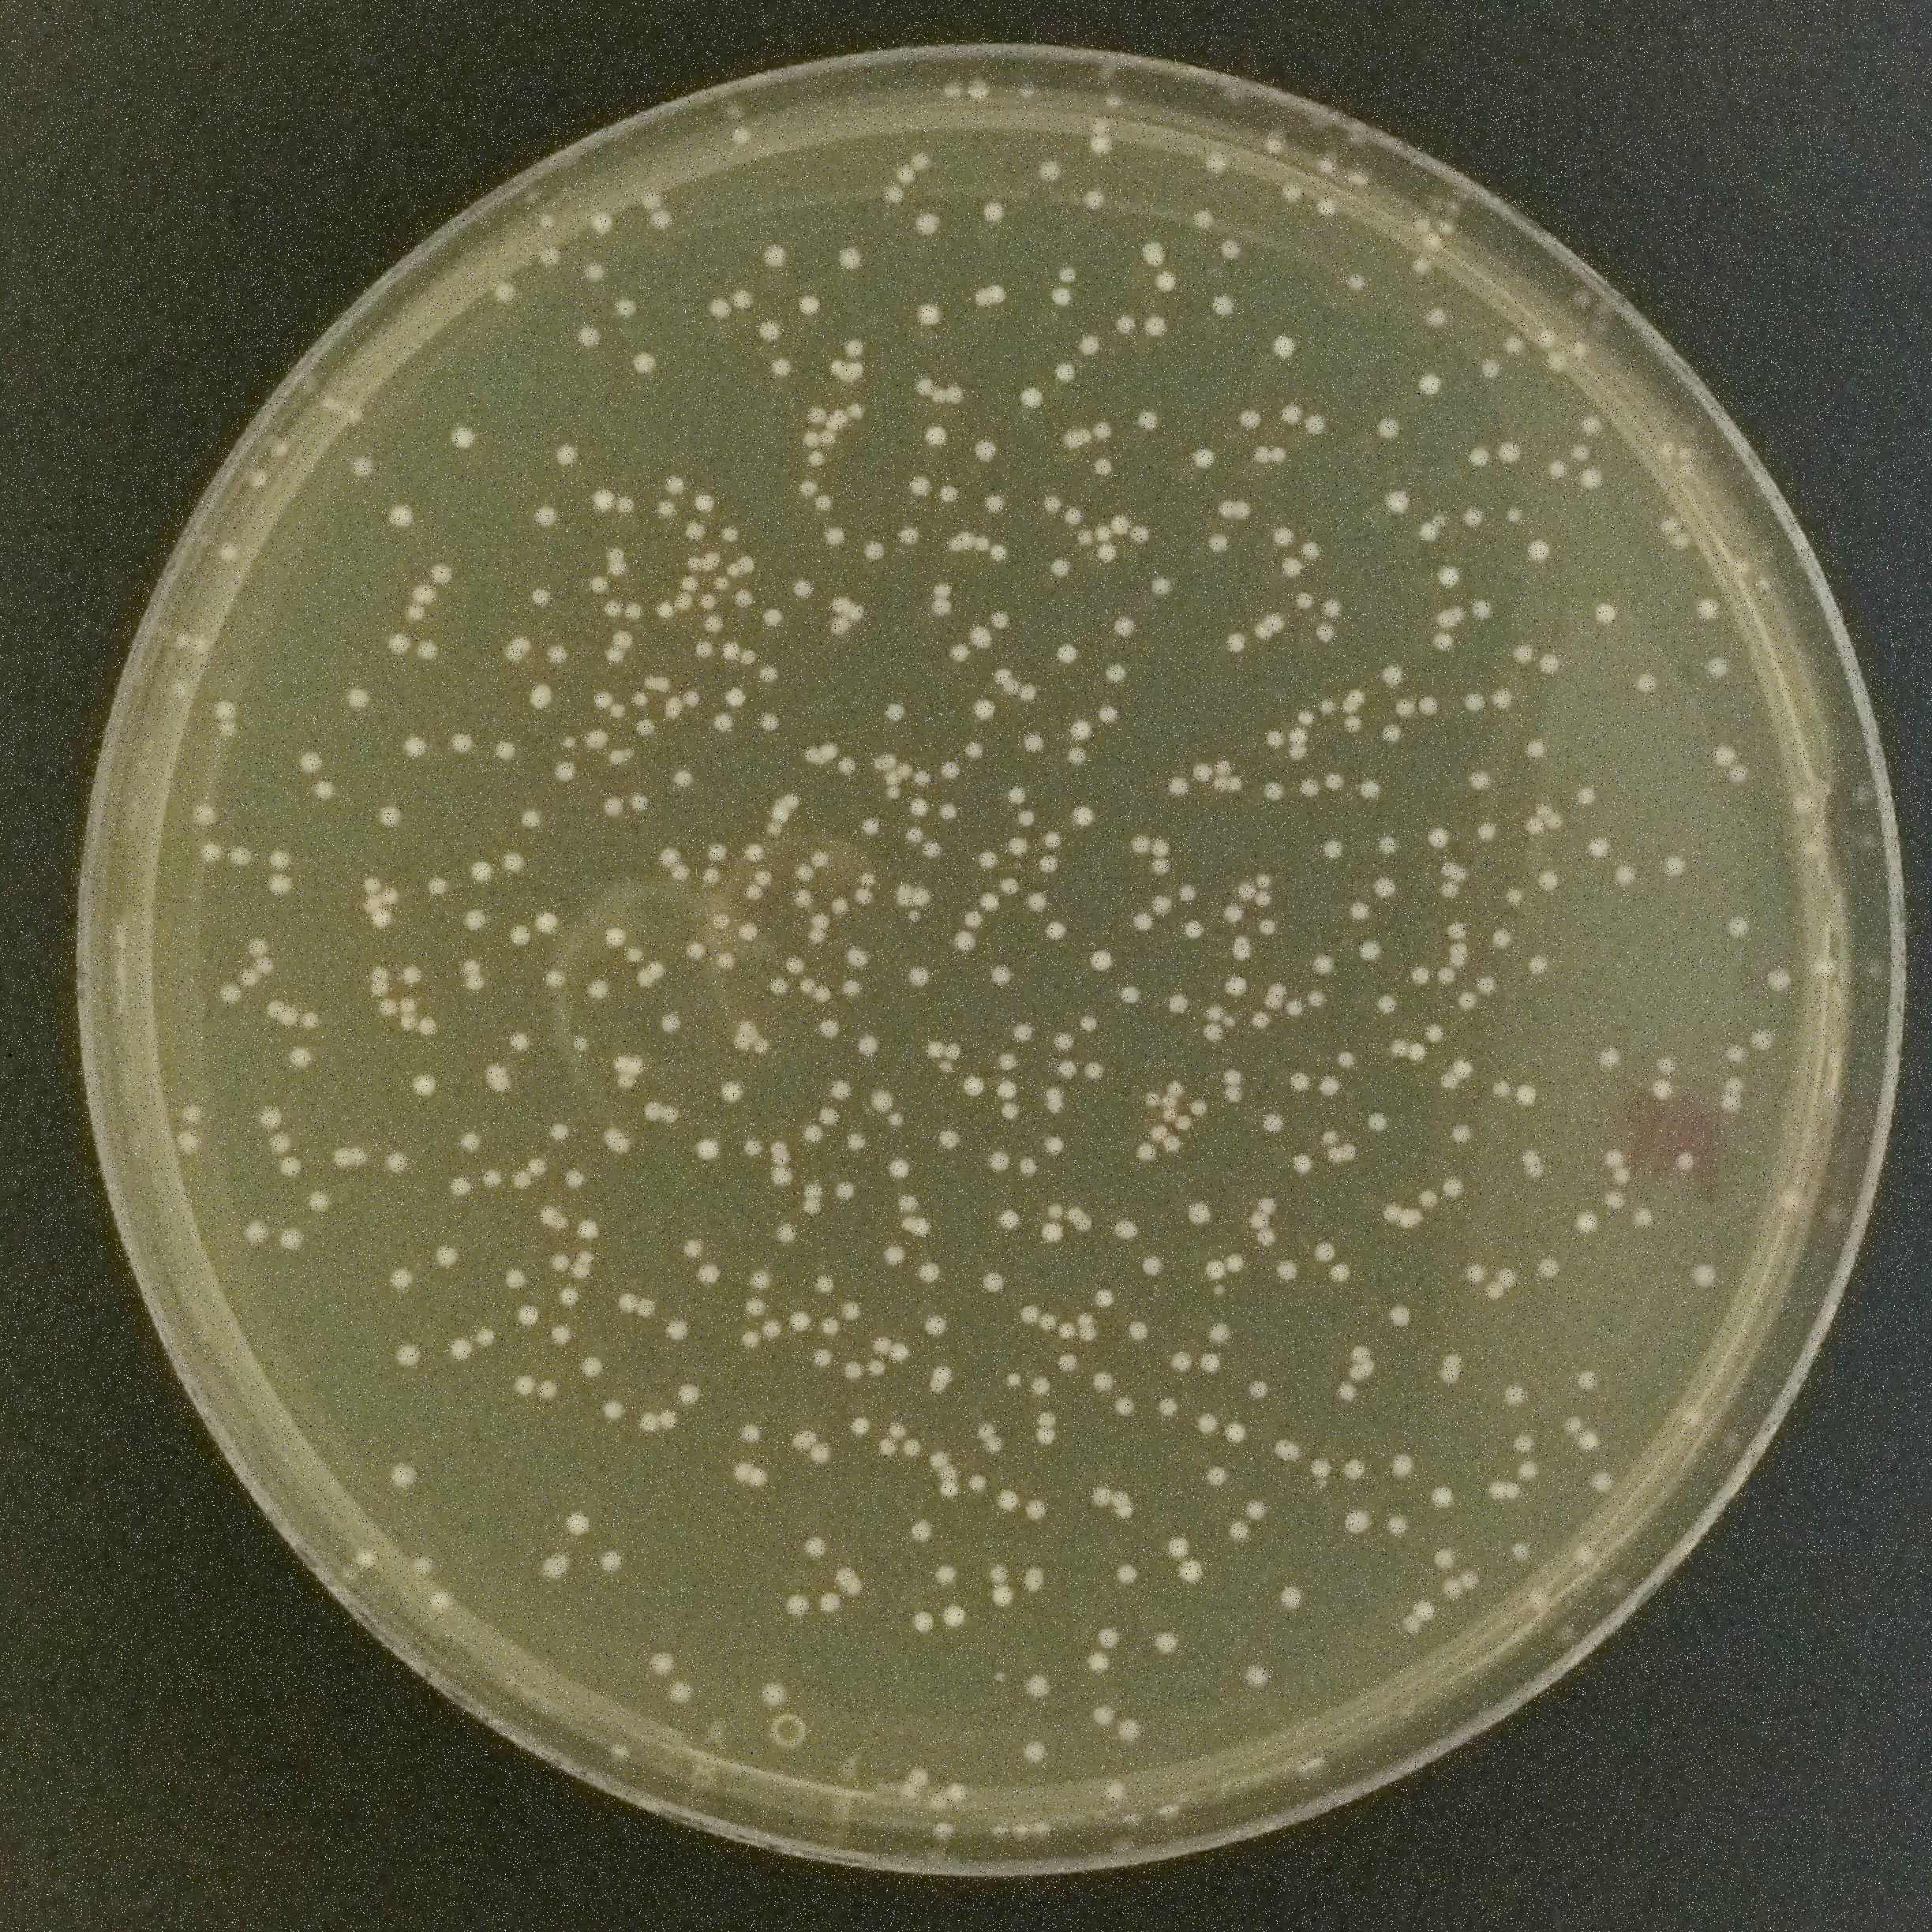
\includegraphics[width=0.25\textwidth,resolution=300]{augmented_easy_0_image}
                    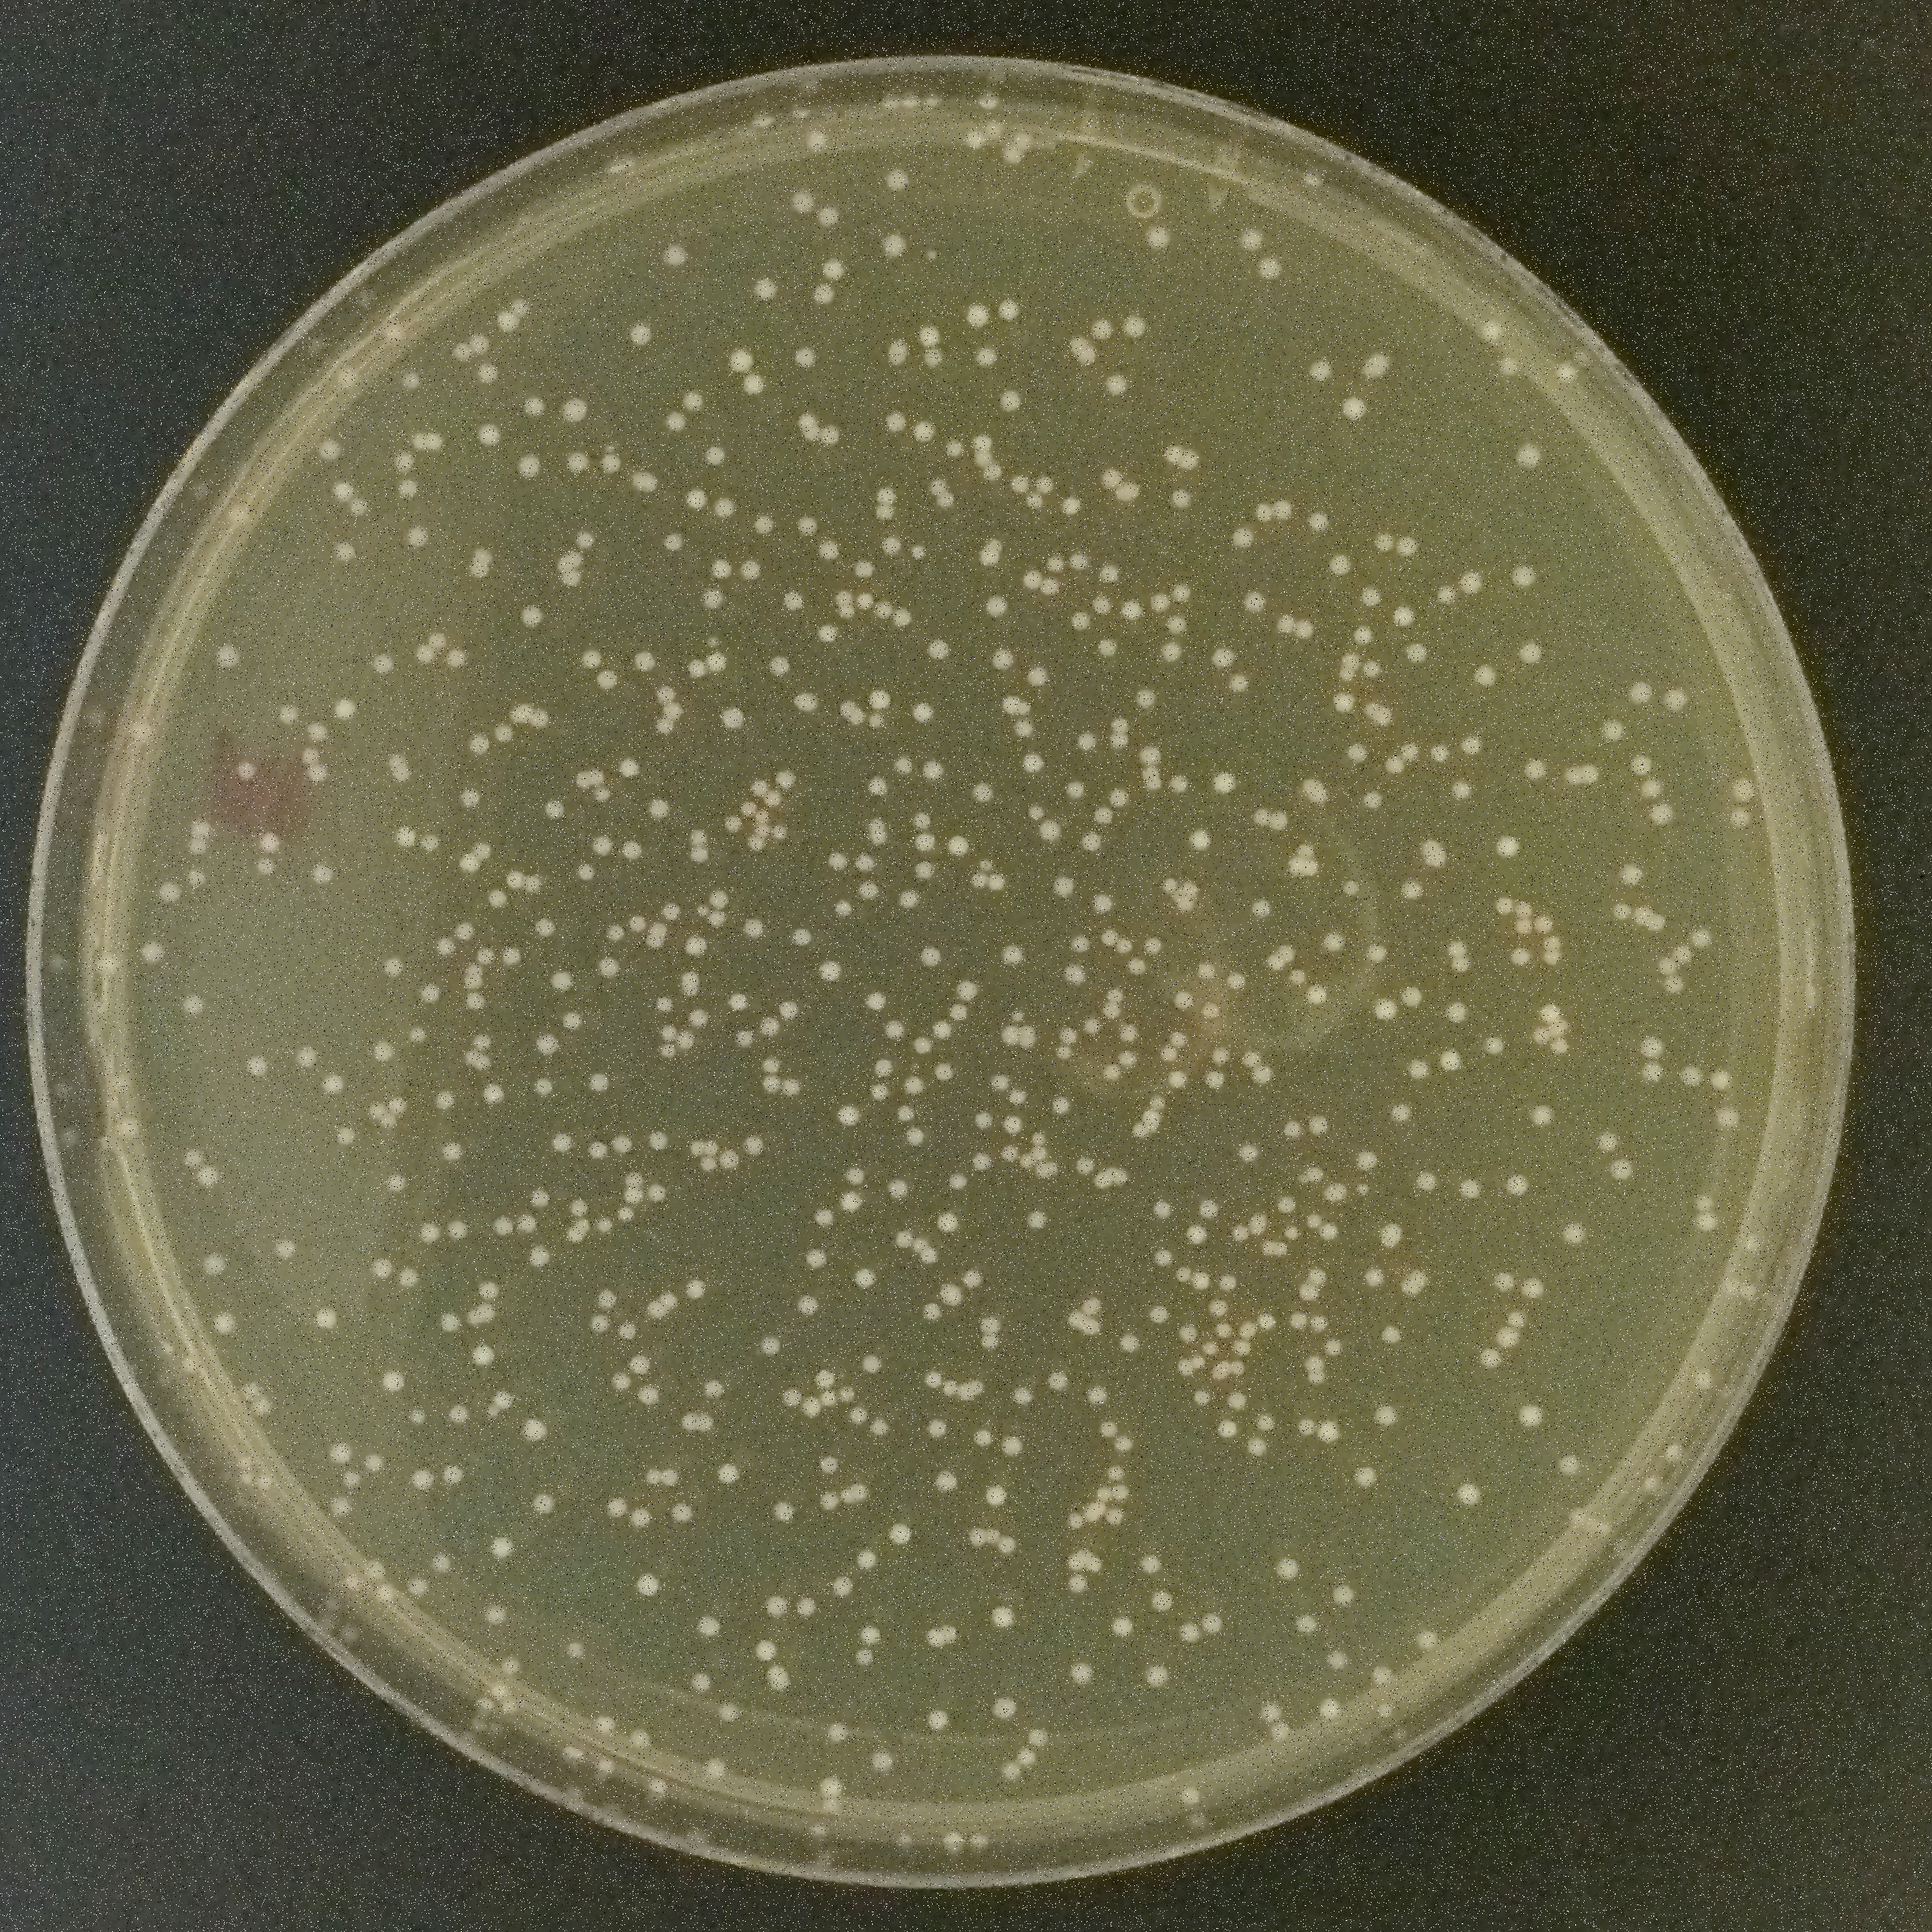
\includegraphics[width=0.25\textwidth,resolution=300]{augmented_easy_1_image}
                    \caption{{\bf Data Augmentation (Mutation).} On the left is an original image. The other two are mutated versions of it.}
                    \label{dcnn_augmentation_mutation}
                \end{figure}
    
            \item
                We then augment the dataset further by duplicating each of the above images $10$ times and rescaling each resulting image by a random factor. An example can be seen in Fig.~\ref{dcnn_augmentation_rescaling}.
    
                \begin{figure}[h]
                    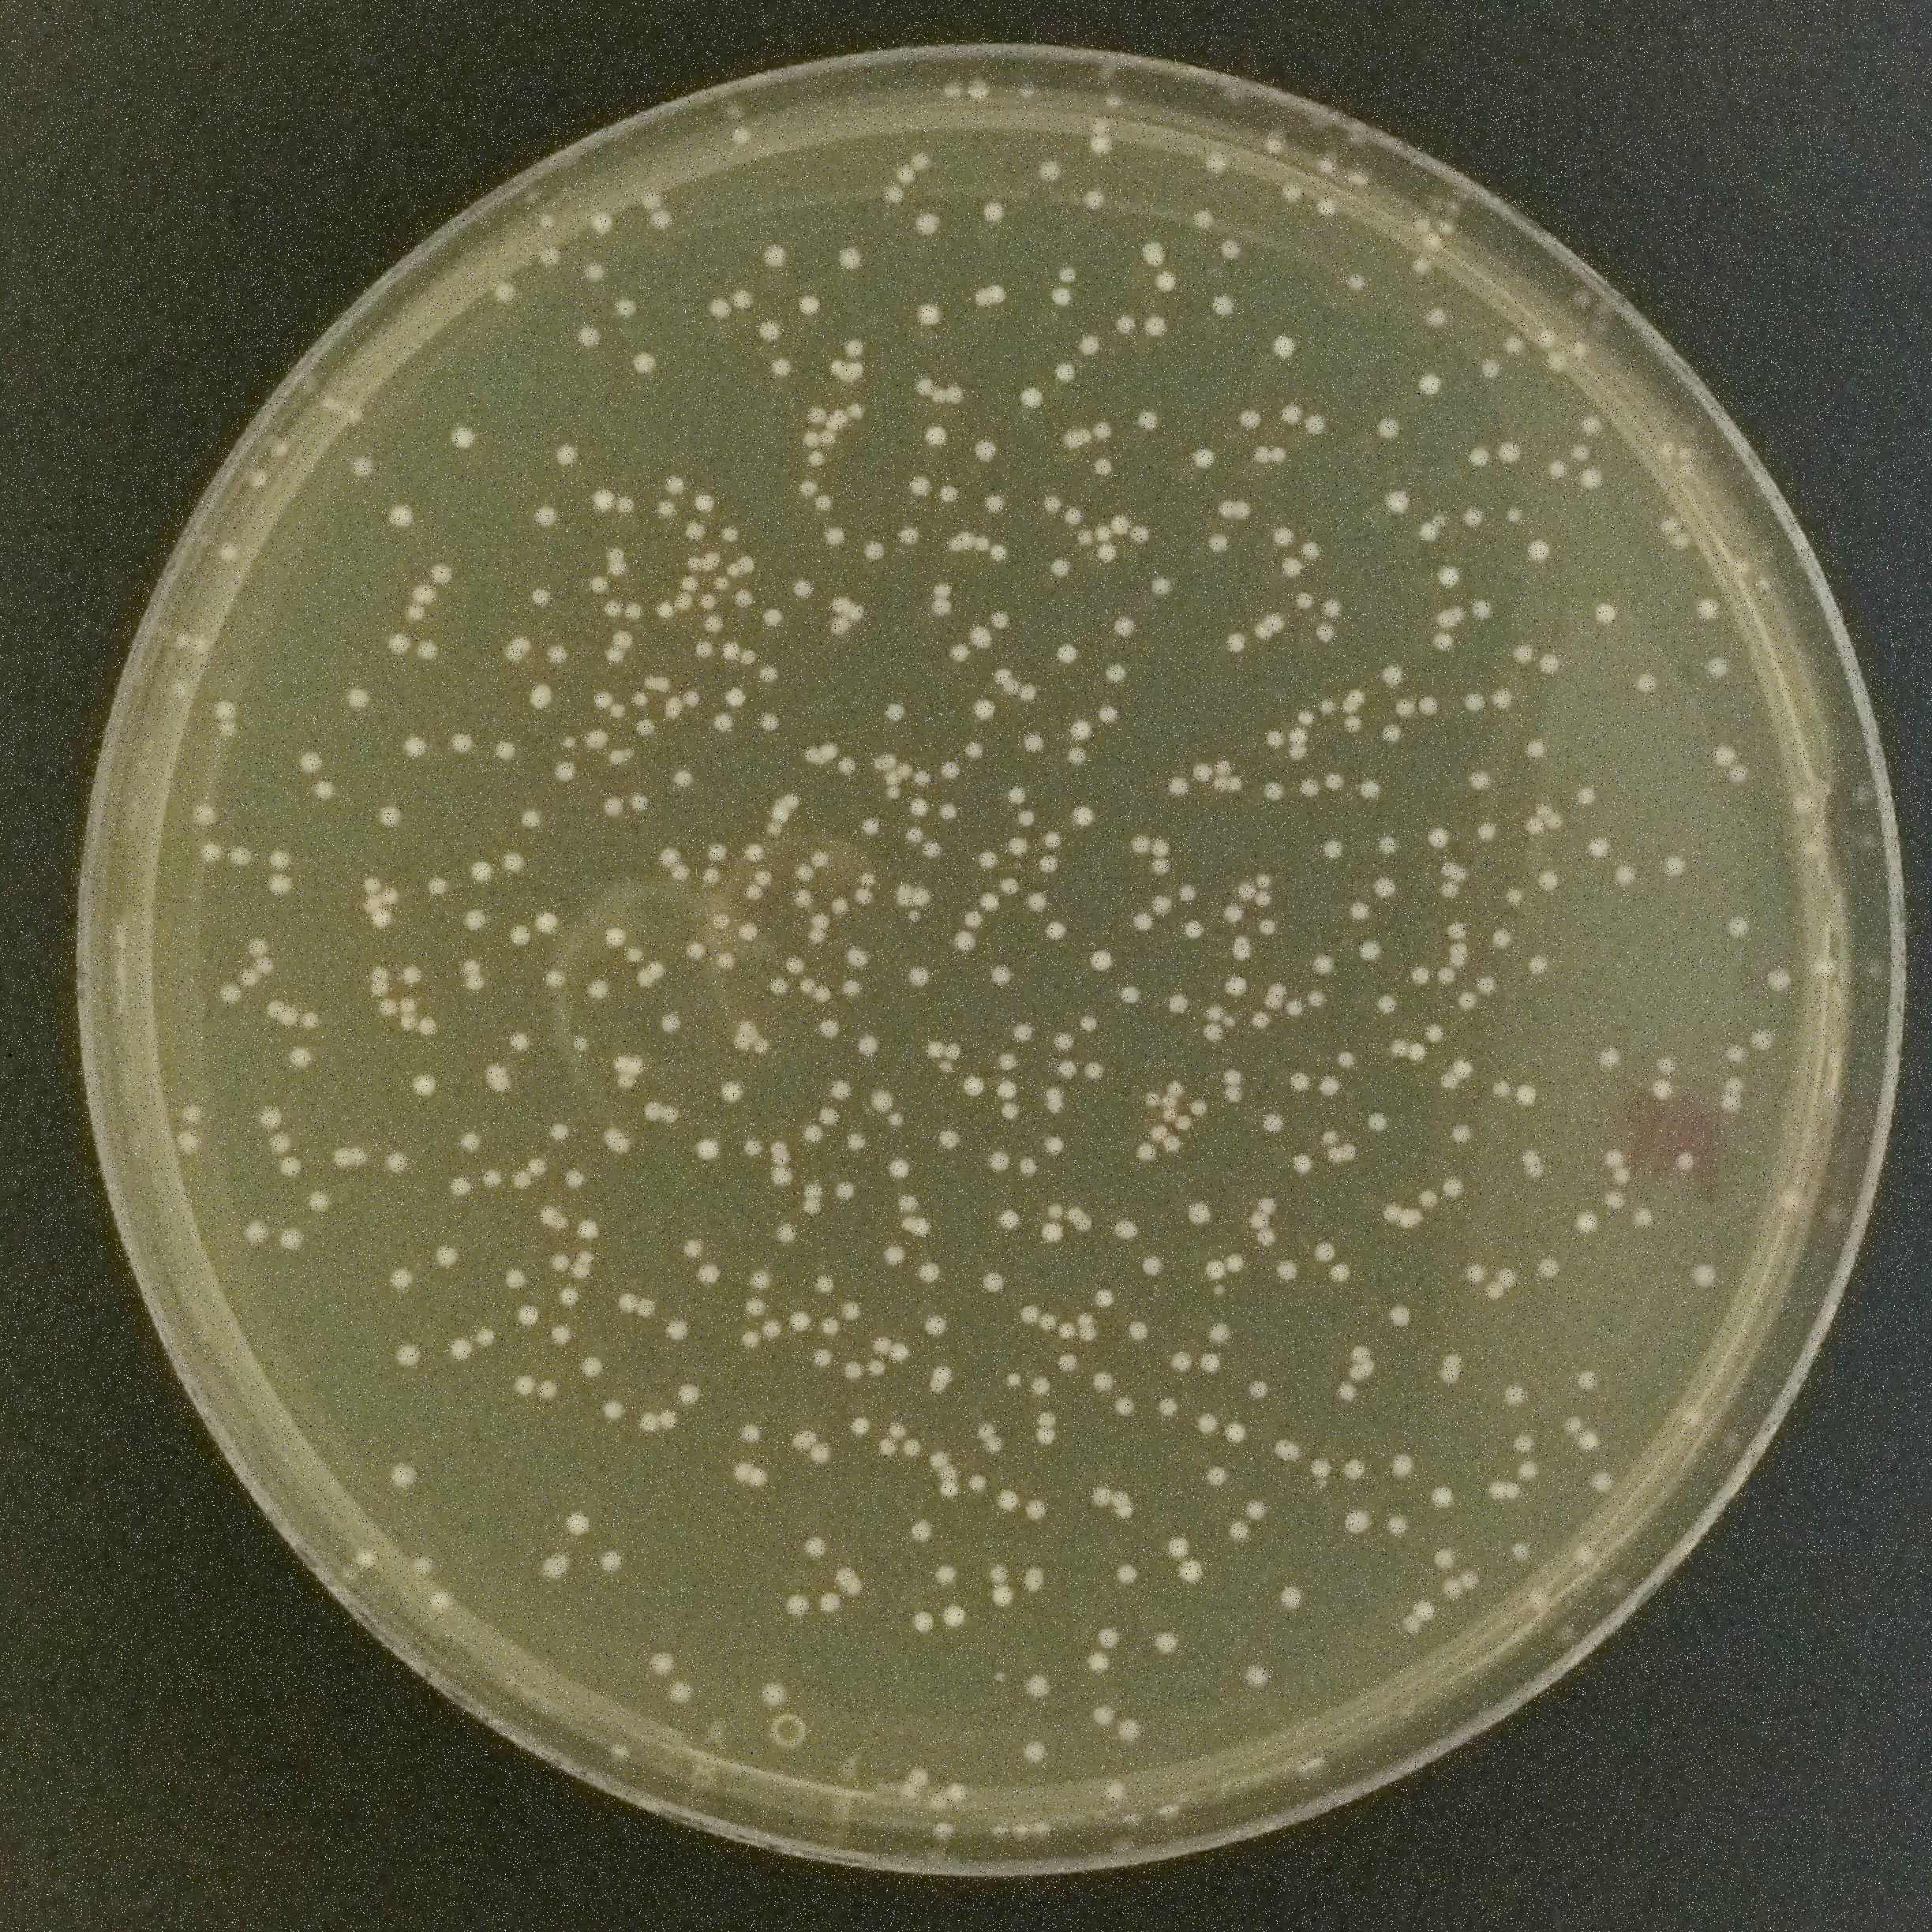
\includegraphics[width=0.25\textwidth,resolution=300]{augmented_easy_0_image}
                    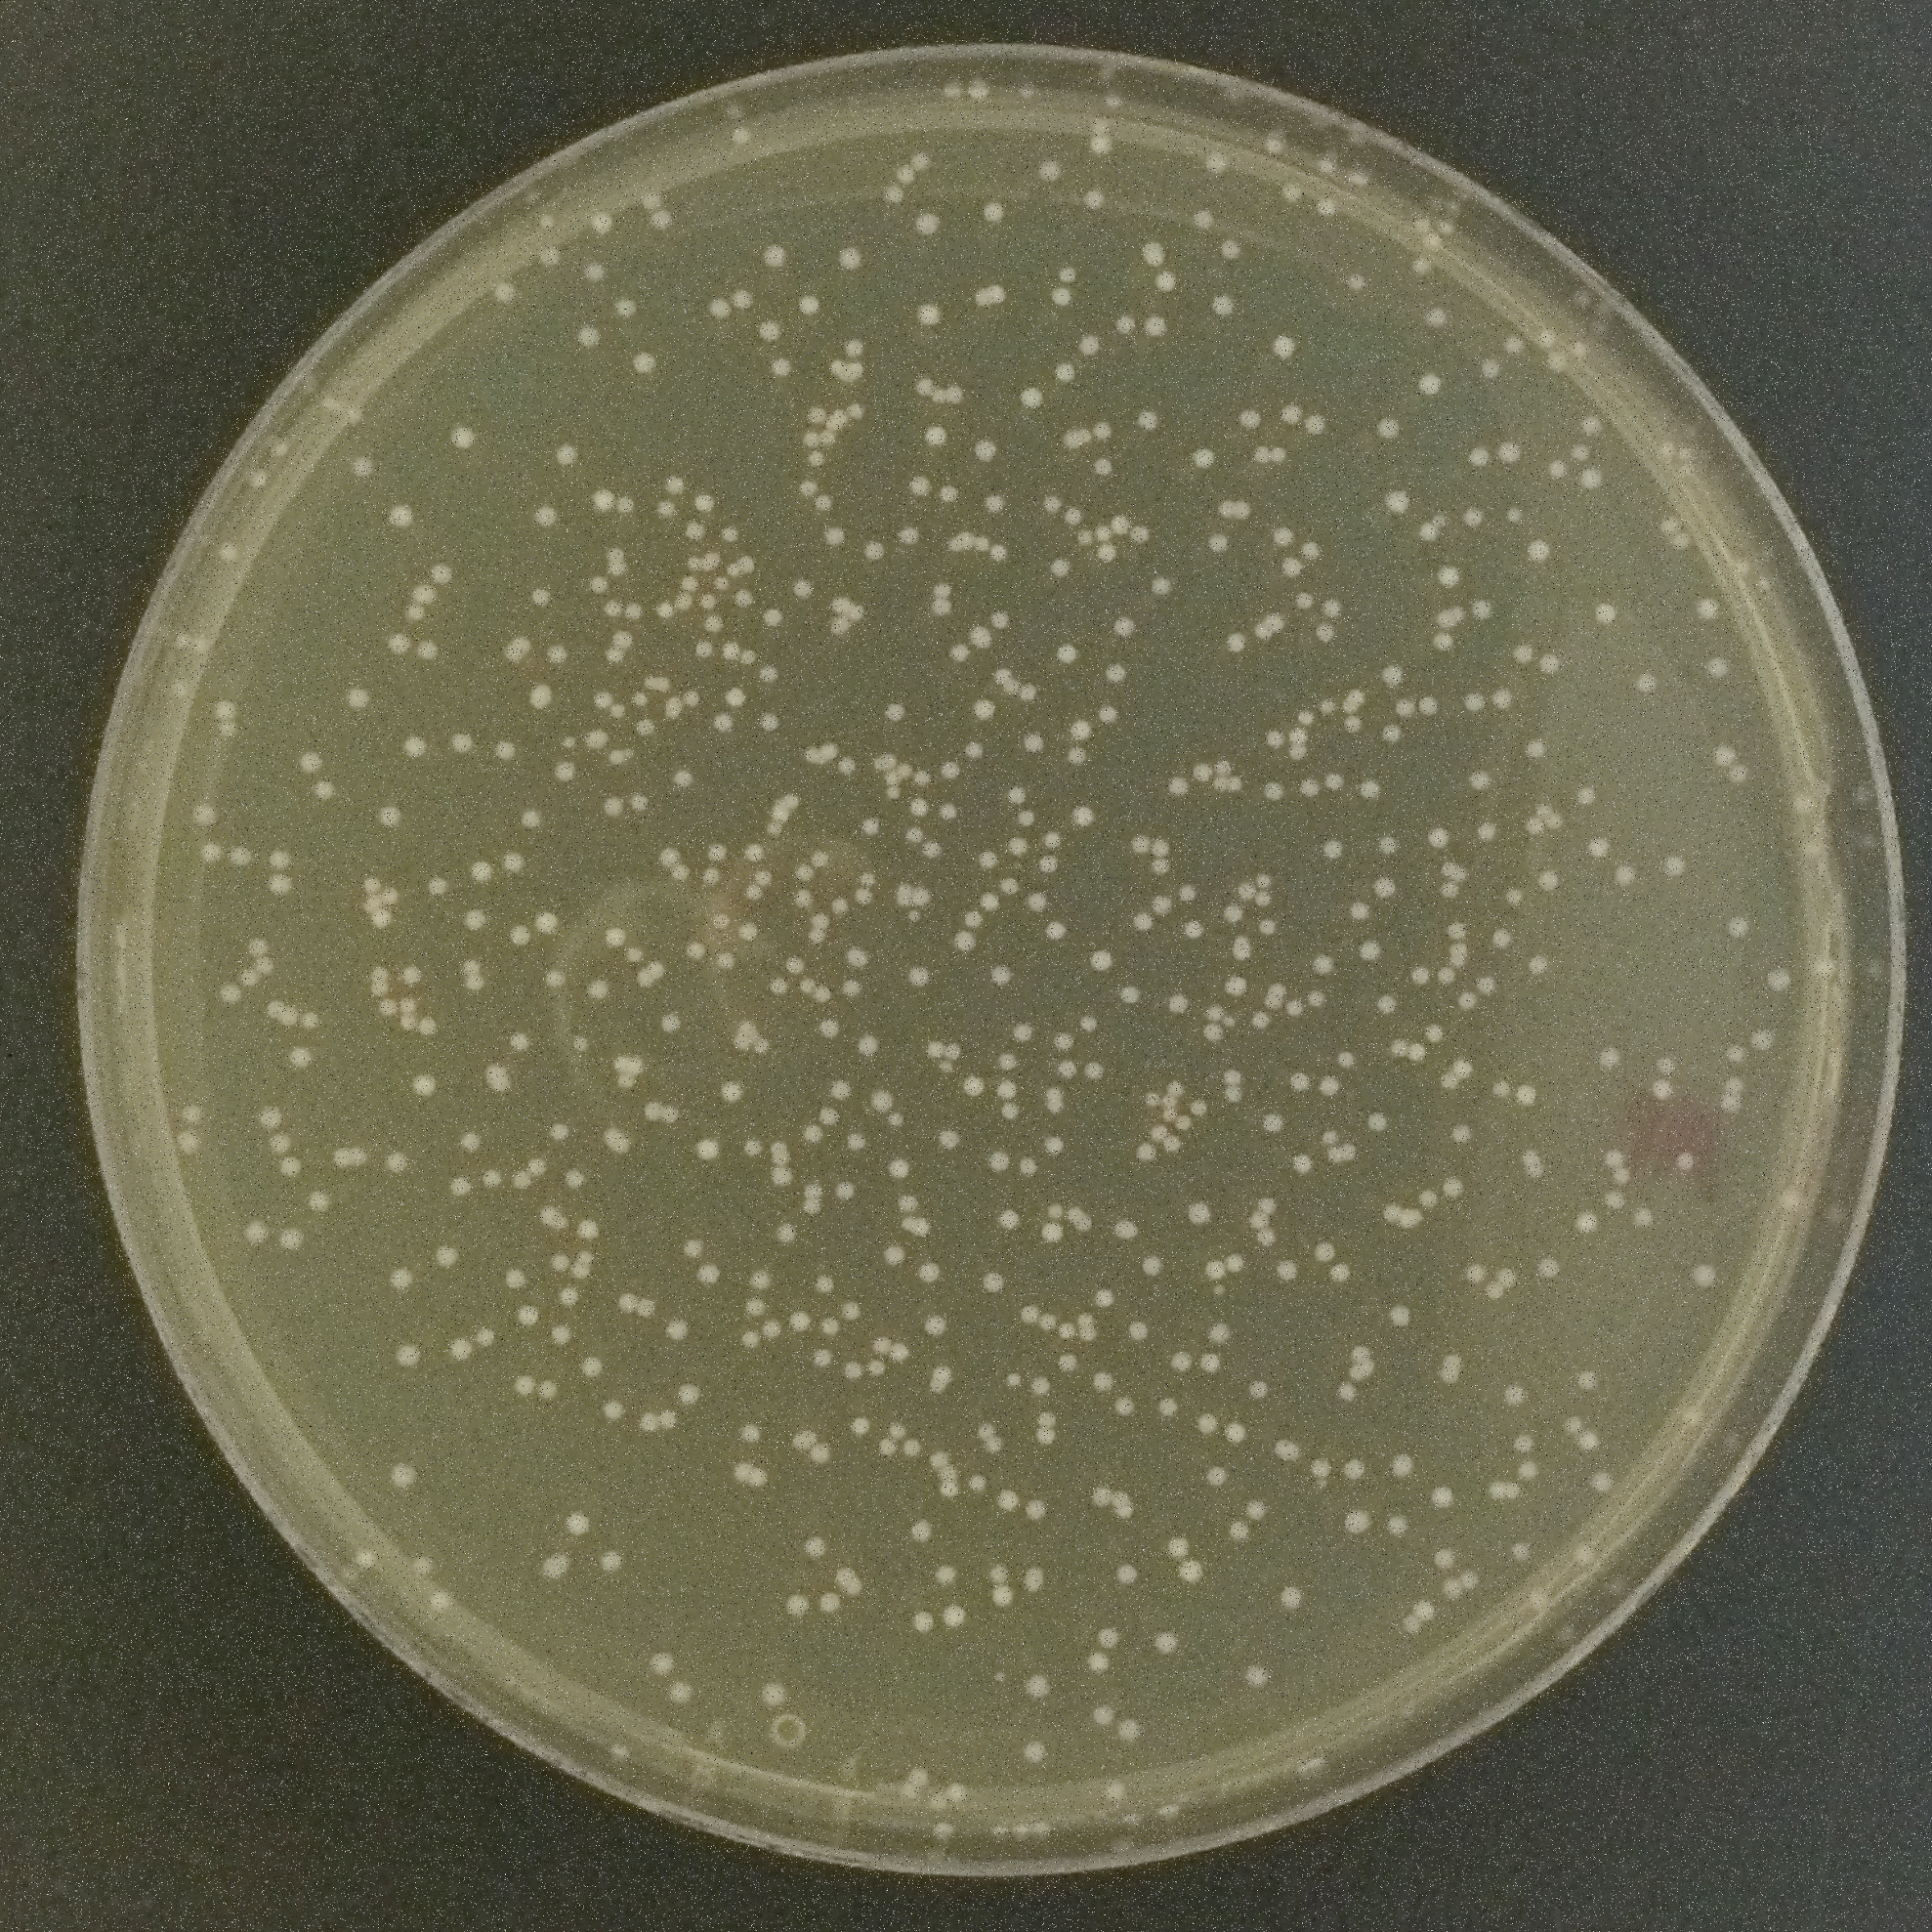
\includegraphics[width=0.18\textwidth,resolution=300]{resized_easy_0_image}
                    \includegraphics[width=0.32\textwidth,resolution=300]{resized_easy_80_image}
                    \caption{{\bf Data Augmentation (Rescaling). On the left is a mutated image from Fig.~\ref{dcnn_augmentation_mutation}. The other two are rescaled versions of it.}}
                    \label{dcnn_augmentation_rescaling}
                \end{figure}

            \item
                We then normalize the images by dividing out their mean pixel values.
        
            \item
                We extract a total of $1,000,000$ patches of dimensions $61px \times 61px$ from the images. We associate a class -- one of \texttt{inside}, \texttt{edge}, or \texttt{outside} -- with each patch. A patch's class describes its center pixel. For example, if its center pixel is \texttt{inside} a CFU according to the masks, then the patch is considered to be of class \texttt{inside}\fxnote{Add a diagram showing this process.}. The patches are sampled such that all classes are represented equally, even if there are far more \texttt{outside} patches than \texttt{inside} or \texttt{edge}, which is the typical case.
        
            \item
                We normalize the patches by subtracting away their median pixel values.
        
            \item
                We split the dataset into two parts: a training dataset containing $90\%$ of the patches and a validation dataset containing the remaining $10\%$.
    
        \end{enumerate}


    \paragraph*{Training}
        We train the model on $64$-patch batches of the training dataset produced during preprocessing, looping over the entire dataset a bit more than once\fxnote{Do a training run that loops over the dataset at least twice.} over the course of about $4$ hours. The current version of the model is saved periodically.

    \paragraph*{Validation}
        The training step saves multiple versions of the model, each from a different point during the training process. To determine which version is best, we assess each model's accuracy (proportion of predicted outputs which are correct) on the validation dataset. We choose the model that achieves the highest accuracy to move forward with. Whereas the patches in the training dataset have been used to improve the models, the patches in the validation dataset are until now unseen by the models and therefore may provide a better measure of how they would perform on unseen data.

 

  \subsection*{SVM} \label{ssec:svm}
        \paragraph*{Summary.}
            Our second model is a support vector machine (SVM). In brief, the model takes as input a $61px \times 61px$ image. It outputs a "class", one of \texttt{0-4}, \texttt{5-9}, \texttt{10-19}, or \texttt{20+}. Our goal is to be able to input a $61px \times 61px$ image of an individual well from a $96$-well plate and have the SVM output whether that well contains $0$-$4$, $5$-$9$, $10$-$19$, or $20+$ CFUs. The classes could be split into finer-grain bins than this, but the model's accuracy would likely decrease due to the increased number and similarity of the classes.
        
        \paragraph*{Model Overview.}
            We present an overview of some key concepts relating to SVMs below. Specific details on the hyperparameter settings used can be found in \nameref{S2_Text}.
            
            \begin{itemize}
                \item \textit{Support Vector Machine.}
                    A support vector machine (SVM) is a mathematical object that accepts some inputs and returns a class. Assuming there are $d$ inputs, the support vector machine seeks to find the hyperplanes in $\mathbb{R}^d$ that best separate the inputs of each class from the inputs of the other classes. These hyperplanes are defined by some tunable parameters called weights. Mathematically, if the input to the SVM were the vector $x$ and the weights for class $k$ were collected in the vector $w_k$, the SVM would compute a score $w_k \cdot x$ for each class and output the class $k$ with the highest score \cite{Hsu}.
                \item \textit{Training.}
                    A SVM is trained using a training dataset of both inputs $\{x_1, \ldots, x_n\}$ and their correct classes $\{y_1, \ldots, y_n\}$. You seek to minimize the sum of squares of the distances by which inputs cross the separating hyperplanes of their correct classes. Since the function to be minimized is quadratic and the constraints are quadratic, the minimum can be found reliably using some standard techniques in quadratic programming.
                \item \textit{Avoiding Overfitting.}
                    In order to avoid overfitting, an SVM seeks not just any weights that separate the classes well, but the weights with the smallest sum of squares \cite{Hsu}. Intuitively, a hyperplane defined by small weights has a relatively simple shape and does not curve too much to accommodate the data points, similar to a low-degree polynomial. In order to provide the SVM further leeway and discourage overfitting the data points, some data points are allowed to cross the separating hyperplane, with a penalty proportional to the distance of the crossing and to a customizable hyperparameter $C$. We train models for $32$ logarithmically-spaced values of $C$ and choose the best model during validation.
            \end{itemize}
            
        \paragraph*{Preprocessing}
            We train, validate, and test the SVM using $\texttt{pinned}$.
        
            \begin{enumerate}
                \item We normalize the images by dividing out their mean pixel values.
        
                \item We convert the images into a form that describes their gradients and edges instead of their raw pixels.\fxnote{Add plot.}
        
                \item We discretize the counts by sorting them into the bins $0$-$4$, $5$-$9$, $10$-$19$, and $20+$.
        
                \item We split the dataset into three parts: a training dataset containing $60\%$ of the patches, a validation dataset containing $20\%$, and a test dataset containing the remaining $20\%$.
            \end{enumerate}

        \paragraph*{Training}
            The model has some tunable settings called hyperparameters. We generate $128$ possible assignments of these hyperparameters and train a model for each possible assignment.

        \paragraph*{Validation}
            The training step produces multiple trained models, each with a different assignment of the hyperparameters. To determine which model is best, we assess each model's accuracy on the validation dataset. We choose the model that achieves the highest accuracy to move forward with.

\section*{Results}
    \subsection*{DCNN} \label{ssec:dcnn_results}
        \paragraph*{Training.}
            As seen in Fig.~\ref{dcnn_convergence}, after $50$ training iterations (about $1$ minute) the DCNN rapidly reaches $86\%$ validation accuracy. After $12,200$ iterations (about $1.5$ hours), the DCNN's validation accuracy begins to level out around $95\%$. Training is continued for a total of $31,050$ iterations (about $4$ hours), with the DCNN's validation accuracy fluctuating around $95\%$.
            
            While the DCNN's accuracy varies more rapidly at first, towards the end of training it is rather stable. This indicates that the iterative optimization procedure responsible for training the DCNN has by the end of training more or less converged into some local minimum of the error function.
            
            At about $15,800$ iterations, the validation accuracy stops rising with the training accuracy, never to resume. Recall that the validation data is never presented to the DCNN for training, so that when we measure the DCNN's prediction accuracy on the validation data, the answer is representative of the DCNN's accuracy on other new, unseen data. In contrast, when we measure the DCNN's prediction accuracy on the training data, the answer is unfairly high because the DCNN has previously been trained on the correct outputs for the training data. The divergence of the validation and training accuracy curves at $15,800$ iterations indicates that by $15,800$ iterations the DCNN has learned all of the patterns it will learn given the training data and model setup that we have chosen. The additional training time is used by the DCNN to "memorize" the training data, not learn generalizable patterns, which can be seen to improve training accuracy but not validation accuracy. This phenomenon is called overfitting.
            
            \begin{figure}[h]
                \includesvg[svgpath=figures/,width=0.7\textwidth]{dcnn_convergence}
                \caption{{\bf Accuracy During Training.} The training process is iterative, unfolding over $31,050$ iterations (about $4$ hours). Depicted is the model's accuracy during the training process on random batches of training data and validation data.}
                \label{dcnn_convergence}
            \end{figure}
        
        \paragraph*{Classification-Based Metrics}
            In the confusion matrices of Fig.~\ref{dcnn_confusion}, we see the types and frequencies of the DCNN's mistakes as it attempts to classify patches as \texttt{inside}, \texttt{outside}, or \texttt{edge}.
            
            The dark diagonal indicates the DCNN's high accuracy; when the true class is \texttt{inside}, it almost always predicts \texttt{inside}, etc. Specifically, the DCNN classifies $4764 / 5000 = 95.28\%$ of the selected training patches correctly and $4724 / 5000 = 94.48\%$ of the selected validation patches correctly.
            
            Most of the DCNN's mistakes involve classifying an \texttt{inside} patch as an \texttt{edge} patch ($121 / 5000 = 2.42\%$ in validation) or an \texttt{edge} patch as an \texttt{inside} patch ($117 / 5000 = 2.34\%$ in validation). These mistakes are to be expected because the outlines that indicate the \texttt{edge} pixels are hand-drawn and somewhat erratic; there is a certain amount of human error in producing the training data that the DCNN cannot predict. These mistakes are also harmless because we are for now only interested in counting; if the DCNN shaves some pixels off the edge of a CFU, this is unlikely to have any affect the count obtained.
            
            The remaining errors ($19 / 5000 = 0.38\%$), while undesirable, are rare. One caveat is that while an \texttt{outside} patch is classified as \texttt{inside} only $3 / 5000$ times ($0.06\%$ of the time) in validation, this effect will be magnified in practice by the fact that the vast majority of pixels in most plate images are \texttt{outside}.
            
            \begin{figure}[h]
                \includesvg[svgpath=figures/,width=0.4\textwidth]{train_confusion_matrix}
                \includesvg[svgpath=figures/,width=0.4\textwidth]{valid_confusion_matrix}
                \caption{{\bf Confusion Matrices.} The cells in column $x$ of a confusion matrix show the DCNN's distribution of predictions for patches of class $x$. On the left, the DCNN is used to classify $5000$ random patches from the training data. On the right, the validation data.}
                \label{dcnn_confusion}
            \end{figure}
        
        \paragraph*{Counting-Based Metrics.}             
            As seen in Fig.~\ref{dcnn_plate_counts}, the DCNN's predicted counts are consistently linear in the actual counts, and would be acceptably accurate after application of a linear transformation ($\text{actual} \approx 1.65(\text{predicted} - 50)$).
            
            \begin{figure}[h]
                \includesvg[svgpath=figures/,width=0.7\textwidth]{predicted_vs_actual}
                \caption{{\bf Predicted Counts vs. Actual Counts (Plates). The DCNN's predicted counts are consistently linear in the actual counts.} \texttt{easy} appears in green, \texttt{more} appears in purple, and \texttt{multi} appears in yellow.}
                \label{dcnn_plate_counts}
            \end{figure}
            
            The differences between the $3$ test datasets counted here, as well as the DCNN's relative accuracy on each, is summarized in Table~\ref{dcnn_plate_summaries}. The consistent linearity of the DCNN's predicted counts appears relatively invariant to negative factors such as CFU size heterogeneity, confluential growth, and poor photographic conditions. This suggests that the DCNN is not brittle; it produces consistent counts, which degrade gracefully when the task is difficult.
            
            \begin{table}[h]
                \begin{adjustwidth}{-1.5in}{0in}
                    \caption{{\bf Relative Count Accuracies.} Each row summarizes a test dataset and the DCNN's relative accuracy on it.}
                    \begin{tabular}{c|l|l|l|r}
                        dataset & CFU size distribution & confluential growth & photographic conditions & count consistency \\
                        \hline
                        \texttt{easy} & homogenous & high & excellent & consistently linear \\
                        \texttt{more} & heterogenous & low & excellent & slightly less consistent \\
                        \texttt{multi} & heterogenous & low & mix of excellent, okay, and poor & slightly less consistent \\
                        \end{tabular}
                    \label{dcnn_plate_summaries}
                \end{adjustwidth}
            \end{table}  

            As seen in Fig.~\ref{dcnn_well_counts}, the DCNN's accuracy in counting individual wells of \texttt{pinned} is poor. While the predicted counts are again linear in the actual, they are too noisy. The issue is likely the low actual count; while the DCNN's estimates are always noisy, when the actual count is low, this noise has a significant effect. Accordingly, we see it become more consistent with increasing actual count.

            \begin{figure}[h]
                \includesvg[svgpath=figures/,width=0.7\textwidth]{well_predicted_vs_actual}
                \caption{{\bf Predicted Counts vs. Actual Counts (Wells). The DCNN's predicted counts are linear in the actual counts, but highly variable.}}
                \label{dcnn_well_counts}
            \end{figure}
            
    \subsection*{SVM} \label{ssec:svm_results}
        \paragraph*{Counts.}
            As seen from the dark diagonal in Fig.~\ref{svm_counts}, the SVM is accurate; it predicts the correct count range for $423$ of the $442$ wells tested ($95.70\%$). The majority of the mistakes it makes involve classifying a "counted" well (classes $1, 2, 3, 4$) as "uncounted" (class $0$). This type of mistake is common among human counters; judging whether the CFUs of a well are separated enough and large enough to bother trying to count is subjective. Furthermore, this type of mistake is not harmful because any wells classified as "uncounted" by the SVM can be rapidly checked for uncountability by humans. The remaining errors, which are harmful, affect only $6$ of the $442$ wells ($1.36\%$).
                        
            \begin{figure}[h]
                \includesvg[svgpath=figures/,width=0.4\textwidth]{confusion_matrix}
                \caption{{\bf Predicted Count Range vs. Actual Count Range. The SVM is used to count $423$ wells comprising the test split of \texttt{pinned}.} The cells in column $lo$-$hi$ of the confusion matrix show the SVM's distribution of predictions for wells whose count is within $[lo, hi)$.}
                \label{svm_counts}
            \end{figure}
        
        \paragraph*{Confidence Cutoffs.}            
            The SVM is capable of outputting for a given input not only its single most likely class, but its probability of being from each class. We calculate the entropy of these probabilities as a measure of the SVM's confidence in the prediction.
            
            If one class has high probability (eg. $1$) and all other classes have low probability (eg. $0$), then the entropy (of the distribution $0, 0, 1, 0, 0$) will be low. If all classes have about equal probability (eg. $0.2$), then the entropy (of the distribution $0.2, 0.2, 0.2, 0.2, 0.2$) will be high. Since in the first case, the SVM's confidence in the prediction was clearly high and in the second case, the SVM's confidence in the prediction was clearly low, it is reasonable in infer that low entropy roughly correlates with high confidence. Accordingly, we use $\text{confidence} = -1 \times \text{entropy}$.
            
            With this confidence metric, we can ignore SVM counts whose confidence is below a set minimum level. While less of the counts will be automated this way, as seen in Fig.~\ref{svm_confidence_accuracy}, the counts that are automated will be more trustworthy; those that are too difficult for the SVM to perform confidently can be turned over to skilled human counters.
            
            \begin{figure}[h]
                \includesvg[svgpath=figures/,width=0.7\textwidth]{accuracy_vs_cutoff}
                \caption{{\bf Retained Count Accuracy vs. Minimum Confidence. By setting an increasingly strict minimum confidence level, we ensure higher and higher accuracy levels for the retained counts.}}
                \label{svm_confidence_accuracy}
            \end{figure}
            
            In rejecting low-confidence counts, we trade some count utilization for some count accuracy. By examining the distribution of confidence levels for the SVM's counts, we can choose a minimum confidence that makes this tradeoff appropriately. For example, considering a minimum confidence of $1.2$, we can look to Fig~\ref{svm_confidence_proportion} to see that about $95\%$ of SVM counts would be retained. We can then look to Fig.~\ref{svm_confidence_accuracy} to see that the accuracy of the retained SVM counts would be about $98.6\%$. Assuming that the remaining $5\%$ of counts are performed correctly by humans, the accuracy of the counts overall would be $98.7\%$. This is significantly improved from the $95.70\%$ accuracy we could expect without analyzing confidence levels.
            
            \begin{figure}[h]
                \includesvg[svgpath=figures/,width=0.7\textwidth]{proportion_vs_cutoff}
                \caption{{\bf Retained Count Proportion vs. Minimum Confidence. By setting an increasingly strict minimum confidence level, we are able to retain a smaller and smaller proportion of the counts.}}
                \label{svm_confidence_proportion}
            \end{figure}

\section*{Conclusion}
    Automated CFU counting expands the realm of feasible experiments and improves data consistency for microbiology research labs. Machine learning techniques such as DCNNs and SVMs perform this task with a level of accuracy that is comparable to human counters'. The models produced for this paper generalize well to new experiments and conditions, allowing labs to take advantage of automated CFU counting without needing the time or expertise to tune a model specifically for their use case.

\section*{Supporting Information}

\subsection*{S1 Text}
\label{S1_Text}
{\bf DCNN Architecture.}  This is a detailed description of the DCNN architecture used in this paper.

\subsection*{S2 Text}
\label{S2_Text}
{\bf SVM Hyperparameters.}  This is a detailed description of the SVM hyperparameter settings considered in this paper.

\section*{Acknowledgments}
\_\_\_

\nolinenumbers

\bibliography{sample}



\end{document}

